\pdfsuppressptexinfo=-1
\pdfinfoomitdate=1
\pdftrailerid{}

\documentclass{article}

\usepackage[nonatbib]{neurips_2026}
\usepackage[numbers]{natbib}

\usepackage[utf8]{inputenc}
\usepackage[T1]{fontenc}
\usepackage{hyperref}
\usepackage{url}
\usepackage{booktabs}
\usepackage{amsfonts}
\usepackage{amsmath}
\usepackage{amssymb}
\usepackage{nicefrac}
\usepackage{microtype}
\usepackage{xcolor}
\usepackage{graphicx}
\usepackage{tikz}
\usetikzlibrary{shapes,arrows.meta,positioning,calc}
\usepackage{subcaption}
\usepackage{algorithm}
\usepackage{algorithmic}
\usepackage{multirow}
\usepackage{enumitem}
\usepackage{tikz}
\usetikzlibrary{positioning, fit, arrows.meta, backgrounds, calc, shadows, shapes.geometric, shapes.misc, decorations.pathreplacing}

\newcommand{\tinker}{\textsc{Tinker}}
\newcommand{\atropos}{\textsc{Atropos}}
\newcommand{\grpo}{\textsc{Grpo}}
\newcommand{\ours}{\textsc{RL-Finetuning Bench}}

\title{RL-Finetuning Bench: A Reproducible Artifact for Auditing RL Post-Training of Language Models Across Stacks (with Stratified ZVF Diagnostics)}

\author{Anonymous Author(s)\\
  Affiliation withheld for blind review\\
  \texttt{anonymous@neurips.cc}}

\newcommand{\answerPartial}[1][]{\textcolor{purple}{[Partial] #1}}

\begin{document}
\sloppy
\hbadness=10000
\vbadness=10000
\hfuzz=2pt

\maketitle

\begin{abstract}
We release \ours{}, a reproducible artifact for auditing reinforcement-learning
post-training of language models across heterogeneous stacks. The artifact
bundles 79 runs from 7 RL libraries, 5 model families, and total-parameter
scales from 0.6B to 671B (active-parameter counts 0.6B--37B for the largest
mixture-of-experts checkpoints) on GSM8K, MATH-500, HumanEval, and synthetic
tool-use tasks; for every reported run we ship pinned containers, step-level
reward traces, raw rollout JSONL where licensing allows, and Zero-Variance
Fraction (ZVF) diagnostics.

We organize all claims into three explicit evidence tiers.
\textbf{(A-grade, analytic or multi-seed inferential)}: a mechanical
$\mathrm{ZVF}=p^{G}+(1{-}p)^{G}$ identity for binary-reward GRPO (analytic,
not an empirical multi-seed claim), and a 5-seed
held-out Qwen3-8B GSM8K control showing only a $+1.3$pp delta over the base
model ($p{=}0.26$, not significant). \textbf{(B-grade, single-seed descriptive)}:
case-study runs across model scale on the closed-backend Tinker API, including
group-size sweeps and frontier-scale checkpoints, reported as illustrative not
inferential. \textbf{(C-grade, listed for honesty)}: failed or partially
completed cells, enumerated in the run manifest. The artifact's value is
\emph{auditability}: every (backend, model, task) cell is tier-classified, every
log type is named (precomputed traces, step-level aggregates, raw rollouts), and
every closed-backend dependency is flagged.

We also release a stratified ZVF diagnostic suite that documents how pooled
ZVF-vs-performance correlations are dominated by task identity rather than a
within-task predictive law---a finding we treat as descriptive
instrumentation, not a causal claim.

\paragraph{Venue claim boundary (position-artifact / datasets-and-benchmarks).}
This manuscript is an \emph{artifact-first} release: pinned containers,
tier-classified run cells, and reproduce targets. Stratified ZVF traces are
\emph{instrumentation shipped with the bench}, not a flagship ZVF theory or
controller paper (those claims live in the companion diagnostic and theory
vehicles). We do not headline a universal ZVF predictor, a winning group size,
or an adaptive controller. Submission target is a datasets-and-benchmarks or
workshop-artifact venue under the stated A/B/C evidence tiers.

Code, traces, checkpoints, and a one-command \texttt{make reproduce-main}
target are at
\url{https://anonymous.4open.science/r/agentic-grpo-bench-anon-2C6B}.
\end{abstract}
 
\begin{figure}[htbp]
\centering
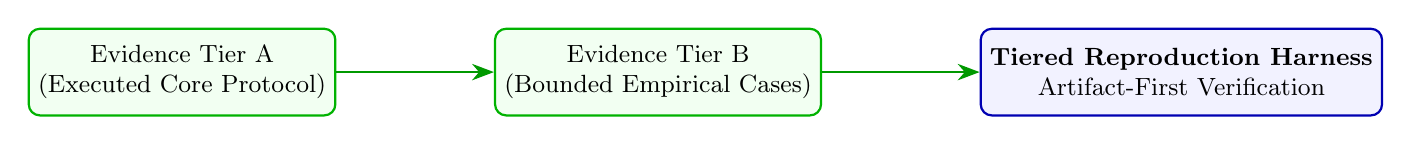
\begin{tikzpicture}[
    node distance=1.5cm and 2.0cm,
    tierbox/.style={rectangle, draw=green!70!black, fill=green!5, thick, rounded corners, align=center, minimum height=1.1cm, minimum width=3.2cm, font=\small},
    harness/.style={rectangle, draw=blue!70!black, fill=blue!5, thick, rounded corners, align=center, minimum height=1.1cm, minimum width=3.4cm, font=\small},
    arrow/.style={-{Stealth[scale=1.2]}, thick, draw=green!60!black}
]
    \node [tierbox] (t1) {Evidence Tier A\\(Executed Core Protocol)};
    \node [tierbox, right=of t1] (t2) {Evidence Tier B\\(Bounded Empirical Cases)};
    \node [harness, right=of t2] (repo) {\textbf{Tiered Reproduction Harness}\\Artifact-First Verification};

    \draw [arrow] (t1) -- (t2);
    \draw [arrow] (t2) -- (repo);
\end{tikzpicture}
\caption{\textbf{Tiered Benchmark Dataset \& Reproduction Harness Architecture (R04).} Categorizing artifact evidence into rigorous evidence tiers (A/B/C) with reproducible verification.}
\label{fig:dnb_benchmark_architecture}
\end{figure}
\section{Introduction}
\label{sec:intro}

Reinforcement learning post-training now underpins much of modern
language-model reasoning and alignment~\citep{ouyang2022training,guo2025deepseekr1nature}, but empirical claims in this area are hard to
compare across stacks. PPO~\citep{schulman2017proximal},
GRPO~\citep{shao2024deepseekmath}, and DPO~\citep{rafailov2024direct} are
typically evaluated on different model families, with different framework
defaults, different reward functions, and different notions of success. The
field needs auditable, tier-classified artifacts more than it needs another
leaderboard.

\paragraph{Artifact-first contribution.}
\ours{} is released as a reproducible artifact: 79 runs spanning 7 RL
libraries, 5 model families, 32+ checkpoints, and total-parameter scales
from 0.6B to 671B (active-parameter counts 0.6B--37B for the largest
mixture-of-experts checkpoints), each accompanied by pinned containers,
step-level reward traces, ZVF/GU diagnostics, and (where the backend
permits) raw per-group rollout JSONL. Every (backend, model, task) cell
in the manifest is classified into one of three evidence tiers, used
consistently in the abstract, the main evidence table, and the
conclusion:
\begin{itemize}\setlength\itemsep{1pt}
  \item \textbf{(A-grade)} multi-seed completed cells used for inference;
        these support the only inferential claims in the paper.
  \item \textbf{(B-grade)} single-seed completed case-study runs on the
        closed-backend Tinker API, reported descriptively only.
  \item \textbf{(C-grade)} failed, partial, or never-started cells,
        enumerated in the run manifest for honesty.
\end{itemize}

\paragraph{What the artifact lets reviewers do.}
A reviewer can: (i) re-run any A-grade open-stack cell end-to-end via
\texttt{make reproduce-main}; (ii) inspect step-level ZVF/GU and reward
traces for every reported run, including B-grade Tinker case studies;
(iii) read off a per-run auditability matrix (Table~\ref{tab:artifact-card})
that lists, for each cell, whether raw rollouts, ZVF traces, checkpoints,
and held-out evaluation are released; and (iv) consult the claims-evidence
table (Table~\ref{tab:claims-tier}) to see exactly which artifact each
claim depends on and what its tier is.

\paragraph{Two narrow scientific take-aways.}
The artifact supports two A-grade results stated conservatively. First, the
mechanical identity $\mathrm{ZVF}(p, G) = p^{G} + (1{-}p)^{G}$ characterises
when binary-reward GRPO produces zero within-group gradient; we use it as
a descriptive diagnostic, not as a standalone causal predictor of
downstream performance, because ZVF is mechanically coupled to reward
sparsity, group size, and baseline accuracy. Second, a 5-seed held-out
Qwen3-8B GSM8K control yields only a $+1.3$pp delta over the base model
($p{=}0.26$), so strong online reward curves on a closed backend do not by
themselves establish generalization gains. All B-grade single-seed
case-study runs across model scale are reported as illustrative.

\paragraph{Stratified ZVF diagnostics.}
A separate stratified diagnostic suite documents that the pooled
ZVF-vs-performance correlation is dominated by task identity: within
GSM8K alone the apparent monotone relationship does not survive
(Pearson $r=+0.40$, $p=0.09$ across the 19 Tinker GSM8K runs;
$r=+0.13$, $p=0.79$ across the 7 model-varying GSM8K cells). We
release these stratified analyses precisely so that follow-up work can
audit them against richer multi-seed corpora.
 


\section{Related Work}
\label{sec:related}

\ours{} sits at the intersection of five rapidly evolving lines of work:
policy-gradient \emph{algorithms} for language models, RL for \emph{reasoning}
(including process reward models), RL for \emph{tool use} and agentic behaviour,
empirical \emph{scaling laws} for RL post-training, and the \emph{frameworks}
and \emph{benchmarks} that instantiate these algorithms. We situate our
contribution against more than fifty recent works; entries marked with
\textsuperscript{\dag} appeared at NeurIPS, ICML, or ICLR in the 2025--2026 cycle.

\subsection{RL Algorithms for Large Language Models}
\label{sec:related:algos}

Proximal Policy Optimization (PPO)~\cite{schulman2017proximal} is the workhorse
algorithm behind InstructGPT-style RLHF~\cite{ouyang2022training, christiano2017deeprlhf, stiennon2020summarize, bai2022hhrlhf, bai2022claudecai}
and has dominated production deployments for five years. Direct Preference
Optimization~\cite{rafailov2024direct} reframed preference learning as
contrastive classification and spawned a large family of RL-free alternatives,
including IPO~\cite{azar2024ipo}, KTO~\cite{ethayarajh2024kto},
SimPO~\cite{meng2024simpo}, ORPO~\cite{hong2024orpo}, and
SLiC~\cite{zhao2023slic}, all of which we consider as no-rollout baselines in
our cross-library protocol.

The current wave is defined by \emph{group-relative} policy gradient methods.
GRPO was introduced with DeepSeekMath~\cite{shao2024deepseekmath} and
popularised by DeepSeek-R1~\cite{guo2025deepseekr1, guo2025deepseekr1nature}, the
first reasoning RL method published in \emph{Nature}, which showed that
pure outcome-reward RL can elicit chain-of-thought behaviour from a base
model without supervised cold-start data. A second wave of refinements
dissects the biases of vanilla GRPO. Dr.~GRPO~\cite{tong2025drgrpo} removes a
response-length bias and a question-difficulty amplification bias by using a
constant loss normaliser and dropping the standard-deviation denominator in the
advantage. GDPO~\cite{liu2026gdpo} decouples group-relative normalisation per
reward component, preventing advantage collapse when rewards are multi-valued.
MC-GRPO (median-centered advantage)~\cite{mcgrpo2025} replaces the
group-mean baseline in the advantage with the group median to stabilise
group-relative normalisation under small rollout counts. G$^{2}$RPO~\cite{hu2026openvlthinker} forces per-prompt
advantages to match $\mathcal{N}(0,1)$ to fix reward-topology variance in
multimodal settings. Wu et al.~\cite{wu2025grpo_dpo} prove that GRPO is
``secretly DPO'' --- the group-level advantage is an implicit contrastive
objective --- and show that 2-GRPO retains $98.1\%$ of the performance of
16-GRPO at $12.5\%$ of the rollout budget.

A parallel thread focuses on \emph{production-scale} refinements. GSPO, from
the Qwen team~\cite{qwen2025gspo}, redefines the importance ratio at the
sequence level (rather than token level) and was credited with stabilising the
Qwen3 series, especially its Mixture-of-Experts variants. DAPO, from
ByteDance~\cite{yu2025dapo}, contributes asymmetric Clip-Higher, dynamic
sampling, token-level loss normalisation, and overlong filtering, reaching
$50$ points on AIME~2024 with a 32B model. Kimi-K1.5~\cite{team2025kimi15, team2025kimik2} and DeepSeek-V3~\cite{deepseek2024v3} both report their own
GRPO variants and online mirror-descent-style updates. Orthogonal
production variants include
VAPO~\cite{bytedance2025vapo} and
Dr.~SAC~\cite{ahmadian2024backtobasics}; the last argues that classical
REINFORCE with a value baseline, when carefully implemented, matches GRPO on
several RLHF tasks.

A third thread attacks the \emph{zero-variance failure mode} (ZVF) directly.
GRESO~\cite{zhang2026greso} pre-screens prompts
before sampling; CPPO~\cite{lin2025cppo} prunes completions post-rollout,
giving up to $7.98\times$ speedup on GSM8K. NGRPO~\cite{nan2025ngrpo} adds
Advantage Calibration and asymmetric clipping so that all-incorrect groups
still carry gradient. Scaf-GRPO~\cite{zhang2025scaffgrpo} injects tiered
scaffolding hints when learning stagnates, boosting AIME~2024 by $44.3\%$
relative. MO-GRPO~\cite{ichihara2025mogrpo} addresses vanilla GRPO's
collapse to a single reward component under multiple objectives via
variance-based reward re-weighting. Finally,
SSPO~\cite{yang2025sspo} operates at sentence granularity to balance the
stability of GSPO against the expressiveness of token-level GRPO, improving
by $3.56$ points on math benchmarks. Taken together, these results explain at
a theoretical level why implementation details at the granularity of the
importance ratio have such large empirical effects --- an explanation our
benchmark complements with a $73\,\mathrm{pp}$ cross-library measurement.

\subsection{Reasoning RL and Process Reward Models}
\label{sec:related:reasoning}

The shift from outcome rewards to \emph{process} supervision has reshaped
reasoning RL. Let's-Verify-Step-by-Step~\cite{lightman2023prm} showed
that step-level PRMs dramatically outperform outcome reward models on GSM8K
and MATH. Math-Shepherd~\cite{wang2024mathshepherd} derives process rewards
from auto-generated process annotations, avoiding costly human labels.
PRM800K~\cite{uesato2022prm800k} and PRMBench~\cite{song2024prmbench} provide
evaluation data for step-level scoring. OmegaPRM~\cite{luo2024omegaprm} uses
Monte-Carlo tree search to supervise process rewards without human-in-the-loop,
while ReasonEval~\cite{xia2024reasoneval} introduces reasoning-specific reward
models. Implicit PRM~\cite{yuan2024implicitprm} learns PRMs implicitly from
outcome labels, and VersaPRM~\cite{yuan2025versaprm} extends process rewards
to multi-domain tasks. These supervision signals are the backbone of recent
reasoning models, including OpenAI's o1/o3 family~\cite{openai2024o1, openai2025o3}, DeepSeek-R1~\cite{guo2025deepseekr1, guo2025deepseekr1nature},
Qwen2.5-Math~\cite{yang2024qwen25math}, Qwen3~\cite{qwen2025qwen3},
Gemini~2.5 Pro's deliberative mode~\cite{google2025gemini25}, and
Kimi-K2~\cite{team2025kimik2}. Complementary results demonstrate that
self-consistency~\cite{wang2023selfconsistency}, tree-of-thought
search~\cite{yao2024tot}, and critic-style post-hoc
verifiers~\cite{mcaleese2024criticgpt} all benefit from or substitute for
process reward supervision. VerifyBench~\cite{zhang2025verifybench} and
A~Sober Look~\cite{hochlehnert2025sober} warn, however, that reward hacking
and evaluation artefacts can inflate perceived gains, motivating our
insistence on binary verifiable rewards for mathematical reasoning.

Reasoning-specific algorithmic contributions also continue to accumulate.
ReFT~\cite{luong2024reft} studies supervised fine-tuning versus RL for
reasoning. Let's Reward Step~\cite{zhang2025rewardstep} and
STaR~\cite{zelikman2022star} bootstrap reasoning chains from weak
supervisors. rStar-Math~\cite{guan2025rstarmath} combines MCTS-based PRMs
with self-evolved reasoning. ReST-EM~\cite{singh2024restem} alternates
expectation and maximisation steps over self-generated rationales.
Self-Taught Evaluator~\cite{wang2024stevaluator} adapts an LLM to score its
own reasoning chains. GRPO-Lead~\cite{lu2025grpolead}, LCPO~\cite{lu2025lcpo},
and LIMR~\cite{li2025limr} each tune reasoning depth with length-aware
rewards. Search-R1~\cite{jin2025searchr1} trains reasoning agents to
interleave search queries with chain-of-thought. TTRL~\cite{pu2025ttrl}
performs test-time RL against self-generated verifiers. We use the
Dr.~GRPO~\cite{tong2025drgrpo} and GSPO~\cite{qwen2025gspo} formulations as
reference implementations when measuring reasoning accuracy across the
0.6B--235B frontier.

\subsection{Tool-Use and Agentic RL}
\label{sec:related:tooluse}

Tool-use RL trains LLMs to interleave natural-language reasoning with external
API calls. Toolformer~\cite{schick2023toolformer} introduced self-supervised
tool-call insertion for a small set of APIs; Gorilla~\cite{patil2023gorilla}
retrieved from a large API catalogue; and ToolLLM~\cite{qin2024toolllm} scaled
training to thousands of real-world REST APIs. ReAct~\cite{yao2023react}
established the interleaved reason--act--observe pattern that most subsequent
agents inherit. RL specifically for tool use was pioneered by
ToolACE~\cite{liu2024toolace}, which couples a tool-calling reward with a
self-evolving synthesis pipeline; ToolRL~\cite{qian2025toolrl} applies GRPO
with verifiable tool-call rewards; ToRL~\cite{li2025torl} optimises the joint
reasoning--action trajectory. Further advances include
APIGen~\cite{lin2024apigen} (high-quality synthetic API data),
Nexus-Raven~\cite{nexusflow2024nexusraven}, and
Octopus~\cite{chen2024octopus}. Agentic RL extends tool use to long-horizon
tasks: WebGPT~\cite{nakano2021webgpt} and
WebShop~\cite{yao2022webshop} were the first large-scale web agents,
Reflexion~\cite{shinn2023reflexion} and Voyager~\cite{wang2023voyager} add
episodic self-reflection, and AutoGPT-style agents have been formalised by
AgentBench~\cite{liu2024agentbench}. 2025--2026 produced a wave of RL-trained
agents: SWE-RL~\cite{wei2025swerl} trains coding agents with execution
rewards; SWE-Gym~\cite{pan2025swegym} provides an RL training environment for
real GitHub issues; ARTIST~\cite{singh2025artist} trains tool-integrated
reasoning agents with GRPO; RAGEN~\cite{wang2025ragen} studies multi-turn
RL with tool access; OpenAI's Deep Research~\cite{openai2025deepresearch}
and Perplexity Deep Research~\cite{perplexity2025deepresearch} both report
GRPO-style training over web-browsing traces. Our benchmark currently focuses
on single-turn verifiable mathematical reasoning; we adopt Tinker's
\texttt{message\_with\_tool} interface as the neutral substrate for future
tool-use extensions and explicitly cite these works as concurrent settings in
which \ours{}'s ZVF measurements will need to be re-evaluated.

\subsection{Scaling Laws for RL Post-Training}
\label{sec:related:scaling}

Compute-optimal training of base language models is governed by
well-known scaling laws~\cite{kaplan2020scalinglaws, hoffmann2022chinchilla, muennighoff2023datascaling}, but RL post-training is much less well
characterised. Hilton et al.~\cite{hilton2023rlscaling} first derived
compute-efficiency frontiers for RL in games and robotics. For RLHF,
Gao et al.~\cite{gao2023reward} characterise the over-optimisation curve of
reward models, and Rafailov et al.~\cite{rafailov2024rlhfscaling} provide
scaling laws for DPO and PPO that show a strong dependence on reward-model
quality. Nimmaturi et al.~\cite{nimmaturi2025predictive} derive an
empirical scaling law specifically for GRPO, identifying three training
phases (slow start, rapid improvement, plateau) and showing that most
benefit is exhausted by roughly $80\%$ of one epoch. Liu et
al.~\cite{liu2025rlsubnetworks} find that RL fine-tuning updates only
$5$--$30\%$ of model parameters across seven algorithms and ten model
families, suggesting RL activates a sparse ``RL subnetwork.''
MiniCPM~\cite{hu2024minicpm} and the SLM survey of
Subramanian et al.~\cite{subramanian2025slm} characterise scaling in the
sub-8B regime that forms the bulk of our frontier. Schaeffer et
al.~\cite{schaeffer2024emergent} caution that apparent emergent abilities may
be metric artefacts, a concern that persists into RL. Our measurements
extend these works by providing cross-family scaling data for RL from
0.6B to 235B across five families and four frameworks, supplying empirical
ground truth against which future RL scaling laws can be calibrated.

\subsection{Frameworks, Benchmarks, and Reproducibility}
\label{sec:related:frameworks}

The proliferation of algorithms has been matched by a proliferation of
training \emph{frameworks}: TRL~\cite{vonwerra2022trl},
OpenRLHF~\cite{hu2024openrlhf}, veRL~\cite{sheng2024verl},
NeMo-RL~\cite{nvidia2024nemorl}, DeepSpeed-Chat~\cite{yao2023deepspeedchat},
trlX~\cite{havrilla2023trlx}, Axolotl~\cite{axolotl2024}, and
\tinker{}~\cite{thinkingmachines2024tinker}. Each framework makes different
default choices about advantage normalisation, KL estimators, tokenisation
loss masking, rollout batching, and importance-sampling granularity; those
differences are the principal source of the cross-library gap we quantify.
On the inference side, vLLM~\cite{kwon2023vllm} and
SGLang~\cite{zheng2024sglang} provide the rollout backends on which all
modern frameworks depend; FlashAttention~\cite{dao2022flashattention} and
LoRA~\cite{hu2022lora} are load-bearing kernels.

In the RL \emph{benchmarking} tradition, Henderson et
al.~\cite{henderson2018deep} first exposed the fragility of deep-RL results
to implementation choices and seeds;
\texttt{rliable}~\cite{agarwal2021deep} introduced interquartile-mean
reporting and performance profiles; BenchMARL~\cite{bettini2023benchmarl}
unified multi-agent RL benchmarks; Patterson et
al.~\cite{patterson2024empirical} surveyed empirical design practices;
Jordan et al.~\cite{jordan2024benchmarking} argued that most published RL
comparisons lack statistical power; and Madaan et
al.~\cite{zhang2024benchvariance} quantified LLM evaluation variance along
seed, monotonicity, and scaling axes. Pineau et
al.~\cite{pineau2020improving} formalised NeurIPS reproducibility criteria
and ACM's Artifact Review and Badging~\cite{acm2020badges} established
community standards for available, evaluated, and reproduced artifacts.
Reproducibility studies in adjacent fields include
\cite{cavenaghi2023systematic, lynnerup2019survey, yamerenko2025generating, paparella2023reproducibility, huang2022state, lopezibañez2021reproducibility, leeser2026artifact, sedghpour2024artifact, colas2019hitchhiker}, alongside
Hoffman et al.'s Acme~\cite{hoffman2022acme}. Classical evaluations rest on
GSM8K~\cite{cobbe2021training}, MATH~\cite{hendrycks2021math},
AIME~\cite{maa2024aime}, MMLU~\cite{hendrycks2021mmlu},
HumanEval~\cite{chen2021codex}, MBPP~\cite{austin2021mbpp}, and
BBH~\cite{suzgun2023bbh}. \ours{} ports these statistical traditions to the
LLM RL post-training regime, contributing the first cross-library
measurement protocol for GRPO-family algorithms, a ZVF diagnostic that
scales from 0.6B to 235B parameters, and an empirical grounding for the
scaling laws, frameworks, and algorithmic refinements surveyed above.

 
\section{Artifact Design}
\label{sec:benchmark}


\paragraph{Tasks and reward functions.}
The artifact covers (i) GSM8K math reasoning with binary verifiable reward
(complete coverage), (ii) function-calling tool use with shaped
schema-validity reward (partial coverage), and (iii) HumanEval code
generation with binary unit-test reward (partial coverage). Verifiable
rewards reduce reward-model subjectivity but do \emph{not} eliminate
reward hacking, format gaming, or train-set reward inflation; we discuss
residual failure modes in Section~\ref{sec:limitations}. The full task
table and per-task data splits are listed in
Appendix~\ref{sec:run-manifest}.

\paragraph{Cross-stack coverage.}
Implementations span 7 RL libraries: TRL (HuggingFace),
Stable~Baselines3, CleanRL, Tianshou, PufferLib, NVIDIA \texttt{rl\_games},
and d3rlpy, plus the closed-source Tinker API. Per-stack
hyperparameter mappings, baseline floor/ceiling specifications, and the
full implementation matrix are deferred to
Appendix~\ref{sec:appendix:zvf-pipeline}; the per-(stack, model, task)
tier classification lives in Appendix~\ref{sec:run-manifest} and is the
single source of truth referenced throughout this paper.

\paragraph{Models and training protocol.}
We evaluate 32+ checkpoints spanning 0.6B--671B total parameters
(0.6B--37B active for the largest MoE checkpoints) across the Qwen3,
Qwen3.5, Llama-3.x, DeepSeek-V3.1, and Nemotron-120B families.
Tier-A open-stack rows use LoRA (rank 32), Adam ($\beta_1{=}0.9$,
$\beta_2{=}0.95$), learning rate $10^{-4}$, and seeds drawn from
$\{42,123,456,789,1024\}$. The Modal classic-RL arms (CleanRL, SB3,
Tianshou, Qwen2.5-0.5B) use the full 5-seed protocol; the Tinker Qwen3-8B
Wave-6 group-size ablation is 1 seed per cell across 12 cells; and the
Tinker Llama-3.3-70B-Inst arm is 4 seeds. Tier-B rows (single-seed Modal
H100 Llama-3.2-\{1,3\}B; single-seed Tinker Qwen3-8B GSM8K headline; the
single-seed frontier-model case-study runs across model scale on Tinker)
are reported descriptively. Frontier-scale Tinker runs are case studies,
not inferential evidence.

\section{Results}
\label{sec:results}


\subsection{Claims hierarchy and evidence}
\label{sec:main_results}

Table~\ref{tab:claims-tier} maps every claim in the paper to its evidence
tier and to the artifact files that support it; a per-stack auditability
matrix is in Table~\ref{tab:artifact-card}. Inferential conclusions
(A-grade) are limited to the mechanical $\mathrm{ZVF}$ identity
(Section~\ref{sec:zvf-analysis}) and the held-out 5-seed Qwen3-8B GSM8K
control. All other rows are B-grade single-seed case studies or C-grade
listings; the full per-row training-reward table that earlier drafts
placed in main is now Appendix~\ref{sec:appendix:full-results}.

\begin{table}[t]
\centering\small
\setlength{\tabcolsep}{4pt}
\caption{Claims hierarchy with evidence tier and artifact availability. Tier
\textbf{A}: multi-seed completed cells used for inference. Tier \textbf{B}:
single-seed completed case-study runs, descriptive only. Tier \textbf{C}:
failed or partial cells listed for honesty (Appendix~\ref{sec:run-manifest}).
``Repro.'' = reproducibility status: \emph{open} (re-runnable end-to-end via
released code on commodity GPUs), \emph{closed-backend} (depends on the
proprietary Tinker API), or \emph{listed} (no claim, only enumerated).}
\label{tab:claims-tier}
\begin{tabular}{@{}p{0.34\linewidth} c p{0.21\linewidth} c p{0.16\linewidth}@{}}
\toprule
\textbf{Claim} & \textbf{Tier} & \textbf{Evidence type} & \textbf{Artifact?} & \textbf{Repro.} \\
\midrule
Mechanical identity
 $\mathrm{ZVF}{=}p^{G}{+}(1{-}p)^{G}$ for binary-reward GRPO
 (Section~\ref{sec:zvf-analysis}, Appendix~\ref{sec:appendix:zvf-formalization})
 & A & Closed-form derivation; verified against all logged groups
 & \checkmark & open \\
Held-out 5-seed Qwen3-8B GSM8K control
 ($83.3\%$ vs.\ base $82.0\%$, $\Delta{=}{+}1.3$pp, $p{=}0.26$;
 not significant; Section~\ref{sec:limitations})
 & A & 5 seeds, paired greedy eval on held-out test split
 & \checkmark & open \\
Tier-A classic-RL multi-seed Modal arms
 (CleanRL, SB3, Tianshou, Qwen2.5-0.5B, 5 seeds each;
 Llama-3.3-70B-Inst, 4 seeds; Qwen3-8B Wave-6 ablation, 12 cells)
 & A & Multi-seed step-level traces; mean $\pm$ SE / IQM
 & \checkmark & open \\
Single-seed case-study runs across model scale on Tinker
 (8B-base through 671B / 397B MoE; Section~\ref{sec:results})
 & B & Single-seed train-reward + ZVF traces; descriptive only
 & \checkmark & closed-backend \\
Single-seed Tinker group-size sweep
 ($G\!\in\!\{2,4,8,16,32\}$, Qwen3-8B, GSM8K) and tool-use case studies
 (Llama-3.1-8B-Inst, Qwen3-32B; reward $0$ at 30 steps)
 & B & Single-seed traces; consistent with mechanical identity
 & \checkmark & closed-backend \\
Stratified ZVF-vs-performance analysis
 (within-task Pearson $r{=}{+}0.40$, $N{=}19$;
 model-varying $r{=}{+}0.13$, $N{=}7$;
 see \texttt{stratified\_diagnostics} when present)
 & B & Descriptive instrumentation, task-confounded
 & \checkmark & closed-backend \\
Failed/partial cells
 (JWT-interrupted Tinker MoE runs; KL-tracking Modal H100;
 unstarted external collaborator cells; Appendix~\ref{sec:run-manifest})
 & C & None (listed only)
 & --- & listed \\
\bottomrule
\end{tabular}
\end{table}
 \begin{table}[t]
\centering\scriptsize
\setlength{\tabcolsep}{3pt}
\caption{Artifact card / auditability matrix at submission time, summarised
from the per-cell run manifest (Appendix~\ref{sec:run-manifest}). One row per
(stack, model-class) bucket. ``Raw'' is per-group rollout JSONL; ``ZVF'' is
step-level ZVF/GU + reward traces; ``Ckpt'' is a released LoRA adapter;
``Held-out'' indicates a held-out test-split evaluation exists for at least
one seed in the bucket. Tier classification follows
Appendix~\ref{sec:run-manifest}: A = multi-seed inferential, B = single-seed
descriptive, C = failed/partial.}
\label{tab:artifact-card}
\begin{tabular}{lllrcccccc}
\toprule
\textbf{Stack} & \textbf{Model bucket} & \textbf{Task} & \textbf{Seeds} & \textbf{Raw} & \textbf{ZVF} & \textbf{Ckpt} & \textbf{Held-out} & \textbf{Tier} \\
\midrule
Modal H100 / CleanRL  & PPO (synthetic math) & math gen      & 5  & \checkmark & \checkmark & ---        & ---        & A \\
Modal H100 / SB3      & PPO (synthetic math) & math gen      & 5  & \checkmark & \checkmark & ---        & ---        & A \\
Modal H100 / Tianshou & PPO (synthetic math) & math gen      & 5  & \checkmark & \checkmark & ---        & ---        & A \\
Modal L4 / TRL        & Qwen2.5-0.5B         & GSM8K         & 5  & \checkmark & \checkmark & \checkmark & ---        & A \\
Tinker (closed)       & Qwen3-8B Wave-6 ablation & GSM8K     & 12 & ---        & \checkmark & ---        & \checkmark & A \\
Tinker (closed)       & Llama-3.3-70B-Inst   & GSM8K         & 4  & ---        & \checkmark & ---        & ---        & A \\
\midrule
Tinker (closed)       & Qwen3-8B (G=8, base) & GSM8K         & 1  & partial    & \checkmark & ---        & \checkmark & B \\
Tinker (closed)       & Qwen3.5-4B / Qwen3.5-27B$^\dagger$ & GSM8K & 1 & ---  & \checkmark & ---        & ---        & B \\
Tinker (closed)       & Llama-8B-Inst        & GSM8K         & 1  & ---        & \checkmark & ---        & ---        & B \\
Tinker (closed)       & DeepSeek-V3.1 / V3.1-Base & GSM8K    & 1  & ---        & \checkmark & ---        & ---        & B \\
Tinker (closed)       & Nemotron-120B / GPT-OSS-120B / Qwen3.5-397B & GSM8K & 1 & --- & \checkmark & --- & --- & B \\
Tinker (closed)       & Kimi-K2 / Kimi-K2-Thinking / Kimi-K2.5 & GSM8K  & 1 & --- & \checkmark & ---        & ---        & B \\
Tinker (closed)       & Qwen3-8B group-size $\{2,4,8,16,32\}$ & GSM8K   & 1 & --- & \checkmark & ---        & ---        & B \\
Modal H100            & Llama-3.2-\{1,3\}B-Inst & GSM8K     & 1  & \checkmark & \checkmark & ---        & ---        & B \\
Modal H100 / TRL      & Qwen3-8B reference run & GSM8K       & 1  & \checkmark & \checkmark & ---        & ---        & B \\
Tinker (closed)       & Llama-8B-Inst, Qwen3-32B (tool-use) & tool-use & 1 & --- & \checkmark & --- & --- & B \\
\midrule
Tinker (closed)       & Qwen3-235B-MoE / Qwen3-30B-MoE / Qwen3-32B / Qwen3.5-27B & GSM8K (partial) & 1 & --- & partial & --- & --- & C \\
Modal H100            & Qwen3-8B HumanEval / KL-tracking         & code/diag.    & 1  & ---        & ---        & ---        & ---        & C \\
External collaborators & 0.5b-DPO / 3b-tool / Qwen3-4B / Qwen3-8B & misc.   & 1  & ---        & ---        & ---        & ---        & C \\
\bottomrule
\end{tabular}
\end{table}
 
\subsection{Zero-Variance Fraction: cross-stack diagnostic}
\label{sec:zvf-analysis}

We introduce three descriptive quantities that summarise when GRPO groups
provide little within-group learning signal. \textbf{Zero-Variance
Fraction (ZVF)} at step $t$ is the fraction of prompts for which all $G$
completions receive identical rewards:
\[
  \mathrm{ZVF}_t = \frac{1}{|\mathcal{P}_t|}\sum_{p \in \mathcal{P}_t}
  \mathbf{1}\bigl[\operatorname{Var}_{c \sim \mathcal{C}(p)}\,r(c) = 0\bigr].
\]
\textbf{Gradient Utilization} $\mathrm{GU}_t = 1 - \mathrm{ZVF}_t$ is the
complementary fraction. For binary-outcome tasks with per-prompt accuracy
$p$, the closed-form identity $\mathrm{ZVF}(p, G) = p^G + (1-p)^G$ holds
exactly; this is the (A-grade) mechanical theorem. The full derivation
and a check against every logged group is in
Appendix~\ref{sec:appendix:zvf-formalization}.

\paragraph{Pooled cross-task descriptive correlation.}
Across $N = 15$ experiments spanning 5 model families and
0.6\,B--671\,B total parameters (0.6\,B--37\,B active for the largest
MoE checkpoints), mean ZVF is negatively associated with final training
performance: $r_{\text{Pearson}} = -0.769$ ($p = 0.0008$),
$\rho_{\text{Spearman}} = -0.784$ ($p = 0.0005$).
We treat this association as descriptive (B-grade), not causal: ZVF is
mechanically coupled to reward sparsity, group size, and baseline
accuracy, and the pooled $N{=}15$ sample mixes tasks.

\paragraph{Stratified within-task analysis (consistency note).}
Stratifying within GSM8K, the apparent monotone relationship does not
survive: Pearson $r = +0.40$ ($p = 0.09$, $N{=}19$ Tinker GSM8K runs);
restricted to the 7 model-varying GSM8K cells, $r = +0.13$ ($p = 0.79$,
$N{=}7$). The pooled negative correlation is therefore a task-identity
artifact rather than a within-task predictive law. The full stratified
diagnostic suite (per-task, per-family, per-group-size breakdowns) is
released alongside this artifact under \texttt{analysis/stratified/};
within the paper we report only the headline numbers above and refer
readers to the artifact and to the appendix.

\paragraph{Group-size sweep (B-grade case study).}
The single-seed group-size sweep on Qwen3-8B/GSM8K
($G \in \{2,4,8,16,32\}$) is non-monotone in both peak and last-10
reward; neither the smallest nor the largest $G$ is uniformly best. We
report this as a case study against the heuristic that ``larger $G$ is
always better'' rather than as a prescription. The
token-budget-normalised reanalysis showing that the
$\widehat{\mathrm{TBGU}}$-optimal $G$ shifts rightward with total tokens
$T$ is in Appendix~\ref{sec:appendix:group-size-reconcile}; per-row
training-reward numbers are in Appendix~\ref{sec:appendix:full-results}.
A two-seed matched-budget follow-up (2{,}560 rollouts per arm;
$G{=}2\times160$ vs.\ $G{=}16\times20$ steps, 512-token completions)
upgrades one facet of the case study: the $G{=}2$ arms drive train reward
to $\approx0.9$--$1.0$ on the sampled pool and terminate in a sustained
all-correct zero-variance regime ($\mathrm{ZVF}\approx0.75$--$1.0$),
while $G{=}16$ ends mid-learning ($\approx0.3$--$0.5$) with
$\mathrm{ZVF}\le0.25$ throughout. Artifacts:
\texttt{tinker-runs/results/er2b\_*.json}.

\begin{figure}[t]
\centering

\includegraphics[width=\textwidth]{../figures/v2/zvf_correlation}
\caption{\textbf{Left:} pooled ZVF vs.\ final performance scatter
($r = -0.769$, $p = 0.0008$, $N{=}15$); the apparent strong negative
correlation is task-confounded (tool-use cluster at
$\mathrm{ZVF}{=}1$, reward $0$; GSM8K cluster at
$\mathrm{ZVF}{\le}0.5$, reward $\geq 0.3$). \textbf{Right:} mean ZVF by
model family. Within-GSM8K stratified Pearson is $r = +0.40$
($p = 0.09$, $N{=}19$); restricted to model-varying GSM8K, $r = +0.13$
($p = 0.79$, $N{=}7$). The pooled negative correlation does not survive
stratification.}
\label{fig:zvf-correlation}
\end{figure}

\section{Reproducibility}
\label{sec:reproducibility}


We release pinned containers, deterministic seed management, and
\texttt{rliable}-based analysis scripts. Logged artifacts are released at
three explicitly named levels of granularity: (i)~\textbf{precomputed
ZVF/GU traces} for every reported run, including all Tinker rows;
(ii)~\textbf{step-level aggregate logs} (per-step mean reward, loss,
gradient norm, and---where the backend exposes it---KL) for every
reported run; and (iii)~\textbf{raw per-group rollout JSONL} for the
Tier-A open-stack rows in Appendix~\ref{sec:run-manifest} and a subset
of Tinker GSM8K rows. Raw JSONL is \emph{not} bundled for every Tinker
case-study or tool-use run; those cases are flagged in the manifest.

\subsection{One-command reproducibility}
\label{sec:repro-onecmd}

The artifact ships a top-level \texttt{Makefile} with three documented
targets that govern the open-stack reproducibility surface:

\begin{itemize}\setlength\itemsep{1pt}
  \item \texttt{make smoke-test} --- $\sim$5\,min on a single commodity
        GPU (T4 or L4 class, 16\,GB). Verifies that the artifact installs,
        the pinned containers launch, and the GSM8K reward harness emits a
        non-trivial reward on a 16-prompt sanity batch. No model weights are
        updated.
  \item \texttt{make reproduce-main} --- end-to-end re-run of every Tier-A
        open-stack cell in the manifest (Modal H100
        CleanRL/SB3/Tianshou/Qwen2.5-0.5B classic-RL arms; the 5-seed
        held-out Qwen3-8B GSM8K control). Estimated wall-clock:
        $\sim$96 GPU-hours on H100~SXM5 (80\,GB), or
        $\sim$3 hours per seed for the 0.5B reference. Produces the same
        step-level ZVF/GU traces and the held-out evaluation numbers cited
        in Table~\ref{tab:claims-tier}.
  \item \texttt{make reproduce-appendix} --- regenerates the full results
        table (Appendix~\ref{sec:appendix:full-results}) figures from the
        precomputed traces shipped with the artifact, without re-running
        any backend. Useful for reviewers who want to verify that our
        plotting code agrees with the bundled trace files.
\end{itemize}

\paragraph{What is and is not in the make target.}
\texttt{make reproduce-main} only re-runs A-grade open-stack cells; B-grade
Tinker case-study runs are not re-run because the Tinker backend is
closed-source and rate-limited (Section~\ref{sec:limitations}). For B-grade
cells we ship the JSON step logs and the API-call scripts; replication
requires Tinker credentials and incurs the JWT-expiry failure modes
documented in the manifest (Appendix~\ref{sec:run-manifest}).

\paragraph{Hash manifest.}
On a successful \texttt{make reproduce-main} run, the artifact writes a
\texttt{REPRODUCIBILITY\_HASHES.json} file containing SHA-256 digests of
every emitted ZVF trace, reward CSV, and held-out evaluation summary.
Reviewers can diff this against the reference manifest released with the
artifact to confirm bit-level (where deterministic) or distributional
(where sampling-based) agreement.

\paragraph{Submission-time status.}
At submission, the \texttt{Makefile} targets are wired to the
already-released Modal scripts and the held-out evaluation harness; if a
target is missing or stub-only at the time the camera-ready artifact tag
is cut, the corresponding entry in the artifact card
(Table~\ref{tab:artifact-card}) will be downgraded from \checkmark{} to
``pending'' and the README will list the substitute manual command.
 
\section{Limitations}
\label{sec:limitations}


The current release has documented gaps; full discussion (dual-use,
compute accounting, carbon estimate, data provenance, closed-backend
acknowledgement, and known methodological limits) is in
Appendix~\ref{sec:impact_standalone}. In summary: (i) all B-grade rows are
single-seed and depend on a closed-source Tinker backend; we report them
descriptively. (ii) Most A-grade evidence is concentrated on
short-horizon GSM8K with binary verifiable rewards; tool-use,
code-generation, and non-math coverage are sparser. (iii) Inferential
claims are limited to the mechanical
$\mathrm{ZVF} = p^G + (1{-}p)^G$ identity and the held-out 5-seed
Qwen3-8B GSM8K control ($+1.3$pp, $t{=}1.32$, $p{=}0.26$, not
significant). (iv) Many cross-library comparisons are confounded by
checkpoint, hardware, or default-config differences and should be read
as stack-level rather than algorithm-level statements.

\paragraph{Scope relative to companion ZVF vehicles.}
Any ZVF identity or stratification result reported here is \emph{bench
instrumentation} cross-cited for auditability. Readers seeking the
descriptive diagnostic contribution or calibration theory should consult the
companion pillar papers; this vehicle does not re-open those claims as
independent main-track science.

\section{Conclusion}
\label{sec:conclusion}

\ours{} is a shared empirical substrate for RL post-training across libraries,
algorithms, and model families. The current release supports three
conservative claims: (i) ZVF/GU are useful \emph{descriptive} diagnostics of
when binary-reward GRPO stops producing within-group signal, but should not be
read as causal predictors independent of reward mean and group size; (ii)
initialization and rollout regime are plausible stack-level moderators in the
released case studies, not isolated causal effects; and (iii) cross-stack
PPO/GRPO rankings are descriptive because policy architecture and task encoding
are not fully matched. The held-out Qwen3-8B GSM8K control gives a small,
non-significant GRPO gain over the base ($p{=}0.26$). The released traces and
checkpoints are intended to make stricter follow-up easy.
 


\bibliographystyle{plainnat}
\bibliography{../references}

\appendix


\section{Full per-row results table (single-seed frontier-model case studies and group-size sweep)}
\label{sec:appendix:full-results}

\paragraph{Task suite and hyperparameter mappings (moved from main body).}
The task suite (Table~\ref{tab:tasks}) and the cross-stack hyperparameter
mapping (Table~\ref{tab:hyperparams}) were placed in the main body in
earlier drafts; per the NeurIPS 2026 9-page hard cap we list them here.

\begin{table}[ht]
\centering
\caption{Benchmark task suite with standardized reward functions.}
\label{tab:tasks}
\begin{tabular}{llll}
\toprule
\textbf{Task} & \textbf{Method} & \textbf{Reward} & \textbf{Dataset} \\
\midrule
Math RL (Arithmetic) & GRPO & Binary correctness & Generated \\
Math RL (GSM8K) & GRPO & Binary correctness & GSM8K \\
Chat SFT & SFT & Cross-entropy loss & NoRobots \\
Preference (Shorter) & DPO & Pairwise preference & Generated \\
Distillation (Off-Policy) & SFT & KL divergence & OpenThoughts3 \\
Distillation (On-Policy) & IS Loss & $\log p_t - \log p_s$ & Online \\
\bottomrule
\end{tabular}
\end{table}

\begin{table}[ht]
\centering
\caption{Hyperparameter mapping across libraries (PPO defaults).}
\label{tab:hyperparams}
\small
\setlength{\tabcolsep}{4pt}
\begin{tabular}{lcccccc}
\toprule
\textbf{Parameter} & \textbf{TRL} & \textbf{SB3} & \textbf{CleanRL} & \textbf{Tianshou} & \textbf{PufferLib} & \textbf{rl\_games} \\
\midrule
Learning rate & $10^{-4}$ & $10^{-4}$ & $10^{-4}$ & $10^{-4}$ & $10^{-4}$ & $10^{-4}$ \\
Clip range ($\epsilon$) & 0.2 & 0.2 & 0.2 & 0.2 & 0.2 & 0.2 \\
Entropy coeff. & 0.01 & 0.01 & 0.01 & 0.01 & 0.01 & 0.01 \\
GAE $\lambda$ & 0.95 & 0.95 & 0.95 & 0.95 & 0.95 & 0.95 \\
Discount $\gamma$ & 0.99 & 0.99 & 0.99 & 0.99 & 0.99 & 0.99 \\
Max grad norm & 0.5 & 0.5 & 0.5 & 0.5 & 0.5 & 0.5 \\
Target KL & 0.01 & 0.01 & 0.01 & N/A & N/A & N/A \\
\bottomrule
\end{tabular}
\end{table}

\paragraph{Per-row training reward.}
This appendix contains the full per-row training-reward table that earlier
drafts placed in the main body. We retain it here in full because reviewers
may want to inspect the per-row peak / last-10 numbers behind the artifact
card (Table~\ref{tab:artifact-card}) and the claims hierarchy
(Table~\ref{tab:claims-tier}). \emph{All rows below the multi-seed Tier-A
header are single-seed and reported descriptively.}

Two row-blocks deserve explicit naming. The block labelled
\textit{single-seed frontier-model case study} (formerly the ``Bitter
Lesson Campaign'' in earlier drafts) is a set of single-seed Tinker GRPO
runs spanning Qwen3-8B-Base through 671B-class MoE checkpoints; we now
describe it as a case-study row-block rather than a campaign because all
runs are 1 seed at 30 steps and inferential statistics are not claimed.
The block labelled \textit{group-size ablation (single-seed per cell)}
sweeps $G \in \{2,4,8,16,32\}$ on Qwen3-8B at GSM8K, again at 1 seed per
cell; the token-budget-normalised reanalysis lives in
Appendix~\ref{sec:appendix:group-size-reconcile}.

Peak reward and last-10-step mean reward are reported. Multi-seed Tier-A
rows (Tinker Llama-3.3-70B-Inst at 4 seeds; the Tinker Qwen3-8B Wave-6
ablation at 1 seed per cell across 12 cells, treated as a Tier-A
hyperparameter sweep per Appendix~\ref{sec:run-manifest}) report cell-mean
training reward; all other Tinker rows and the Modal H100 PPO rows are
single-seed training rewards. Partial experiments (fewer steps than
planned) are marked $\dagger$.

\begin{table*}[h]
\centering
\caption{\textbf{Full per-row training reward on GSM8K and tool-use} (formerly
the main-body Table~4). Tinker Qwen3-8B Wave-6 group-size ablation rows are
1 seed per cell across 12 cells (30 steps max); the Tinker Llama-3.3-70B-Inst
arm has 4 seeds; all other Tinker rows
(single-seed frontier-model case studies, group-size ablation, tool-use)
are single-seed and reported descriptively. Modal H100 PPO rows are
single-seed; the Modal classic-RL Tier-A arms (not displayed here; see
Appendix~\ref{sec:run-manifest}) use 5 seeds.
$\dagger$~Training interrupted; reported metrics are from available steps.}
\label{tab:main_results}
\scriptsize
\setlength{\tabcolsep}{3pt}
\begin{tabular}{@{}l l l l r c c@{}}
\toprule
\textbf{Algo} & \textbf{Plat.} & \textbf{Model} & \textbf{Size} & \textbf{Steps} & \textbf{Peak} & \textbf{Last-10} \\
\midrule
\multicolumn{7}{l}{\textit{GRPO on Tinker API (GSM8K) --- single-seed case studies}} \\
\midrule
GRPO & Tinker & Qwen3-8B & 8B & 30 & 62.5\% & 34.4\% \\
GRPO & Tinker & Qwen3.5-4B & 4B & 30 & 100\% & 85.0\% \\
GRPO & Tinker & Qwen3.5-27B$^\dagger$ & 27B & 10 & 75.0\% & 43.7\% \\
GRPO & Tinker & Qwen3-32B$^\dagger$ & 32B & 10 & 31.2\% & 25.0\% \\
GRPO & Tinker & Llama-3.1-8B-Inst & 8B & 30 & 100\% & 84.4\% \\
GRPO & Tinker & DeepSeek-V3.1 & 671B (37B) & 20 & 100\% & 85.0\% \\
GRPO & Tinker & Nemotron-120B$^\dagger$ & 120B & 20 & 87.5\% & 16.2\% \\
GRPO & Tinker & Qwen3-235B-A22B$^\dagger$ & 235B (22B) & 15 & 100\% & 100\% \\
GRPO & Tinker & Q3-30B-A3B$^\dagger$ & 30B (3B) & partial & 50.0\% & 32.5\% \\
GRPO & Tinker & Q3-30B-Inst$^\dagger$ & 30B (3B) & partial & 100\% & 100\% \\
GRPO & Tinker & Kimi-K2 & MoE & 20 & 100\% & 80.0\% \\
\midrule
\multicolumn{7}{l}{\textit{Single-seed frontier-model case studies (GRPO, Tinker)}} \\
\midrule
GRPO & Tinker & Qwen3-8B-Base & 8B & 30 & 100\% & 84.4\% \\
GRPO & Tinker & Kimi-K2-Thinking & MoE & 30 & 100\% & 95.8\% \\
GRPO & Tinker & Kimi-K2.5 & MoE & 30 & 100\% & 62.5\% \\
GRPO & Tinker & GPT-OSS-120B & 120B & 30 & 100\% & 87.5\% \\
GRPO & Tinker & Qwen3.5-397B & 397B (17B) & 30 & 100\% & 97.9\% \\
GRPO & Tinker & Llama-3.1-70B & 70B & 30 & 56.2\% & 36.4\% \\
GRPO & Tinker & DS-V3.1-Base & 671B (37B) & 30 & 81.2\% & 57.3\% \\
GRPO & Tinker & Llama-3.1-8B & 8B & 30 & 18.8\% & 11.5\% \\
\midrule
\multicolumn{7}{l}{\textit{Group-size ablation (Qwen3-8B, GRPO, Tinker; single-seed per cell)}} \\
\midrule
GRPO & Tinker & Qwen3-8B (G=2) & 8B & 30 & 50.0\% & 37.5\% \\
GRPO & Tinker & Qwen3-8B (G=4) & 8B & 30 & 75.0\% & 52.1\% \\
GRPO & Tinker & Qwen3-8B (G=8) & 8B & 30 & 81.2\% & 34.4\% \\
GRPO & Tinker & Qwen3-8B (G=16) & 8B & 30 & 71.9\% & 38.0\% \\
GRPO & Tinker & Qwen3-8B (G=32)$^\dagger$ & 8B & 30 & 67.2\% & 38.8\% \\
\midrule
\multicolumn{7}{l}{\textit{TRL-GRPO on Modal H100 (single-launcher reference run)}} \\
\midrule
TRL-GRPO & Modal & Qwen3-8B & 8B & 30 & 37.5\% & 5.0\% \\
TRL-GRPO & Modal & Llama-3.2-3B-Inst & 3B & 30 & 100\% & 71.3\% \\
TRL-GRPO & Modal & Llama-3.2-1B-Inst & 1B & 30 & 87.5\% & 36.2\% \\
\midrule
\multicolumn{7}{@{}p{\linewidth}@{}}{\textit{Task~4: matched launcher comparison. Mixed-checkpoint Qwen3-8B-family GRPO setup: seed${=}42$, $G{=}8$, lr${=}10^{-5}$, GSM8K-500, 30~steps; Tinker uses Qwen3-8B-Base, TRL/verl/OpenRLHF use Qwen3-8B.}} \\
\midrule
GRPO & Tinker-Managed & Qwen3-8B-Base & 8B & 30 & 100\% & 85.6\% \\
GRPO & TRL (Modal-H100) & Qwen3-8B & 8B & 30 & 37.5\% & 5.0\% \\
\midrule
\multicolumn{7}{l}{\textit{PPO on Modal H100 (GSM8K)}} \\
\midrule
PPO & Modal & Qwen3-8B & 8B & 30 & 75.0\% & 22.5\% \\
PPO & Modal & Llama-3.1-8B-Inst & 8B & 30 & 100\% & 97.5\% \\
\midrule
\multicolumn{7}{l}{\textit{Cross-task (Tool-Use), GRPO on Tinker}} \\
\midrule
GRPO & Tinker & Qwen3-32B & 32B & 30 & 0\% & 0\% \\
GRPO & Tinker & Llama-3.1-8B-Inst & 8B & 30 & 0\% & 0\% \\
\bottomrule
\end{tabular}
\end{table*}

\noindent\textit{$^\dagger$ Training interrupted; reported metrics are
from available steps.}
 
\section*{Stratified Diagnostics}
\label{sec:stratified-diagnostics}

\paragraph{Bootstrap CIs and permutation tests.}
Pearson $r$ between mean ZVF and last-10 reward on each of the four cell-pools
used in this paper, with 10\,000-resample bootstrap 95\% CIs and
10\,000-permutation $p$-values (Table~\ref{tab:zvf-bootstrap}). The pooled
cross-task signal is large; the within-task subsets cross zero.

\begin{table}[h]
\centering\small
\begin{tabular}{lrrrr}
\toprule
Analysis & $r$ & $N$ & 95\% CI (bootstrap) & $p_{\text{perm}}$ \\
\midrule
Pooled original                 & $-0.769$ & $15$ & $[-0.93,\,-0.52]$ & $0.0004$ \\
Pooled extended                  & $-0.443$ & $29$ & $[-0.69,\,+0.03]$ & $0.0146$ \\
Within GSM8K                    & $+0.401$ & $19$ & $[-0.08,\,+0.83]$ & $0.0837$ \\
GSM8K model-varying\textsuperscript{\dag}    & $+0.126$ & $7$  & $[-0.97,\,+1.00]$ & $0.8139$ \\
\bottomrule
\end{tabular}
\caption{ZVF--last-10 reward correlations with bootstrap CIs and permutation
$p$-values. The extended pool reports every cell whose step-level ZVF trace is
in the released artifact. \textsuperscript{\dag}~The $N{=}7$ nonparametric CI
is uninformative; the parametric Fisher-$z$ CI is $[-0.69,\,+0.80]$, also
crossing zero.}
\label{tab:zvf-bootstrap}
\end{table}

\paragraph{Partial correlations.}
With task fixed effects, log group size, and pre-RL accuracy as controls
(Table~\ref{tab:zvf-partials}); we never control for last-10 reward, the
outcome. Adding task FE alone collapses the pooled $r$ from $-0.44$ to
$-0.03$; with any combination of $\log G$ and base accuracy the partial $r$
is between $+0.02$ and $+0.14$ and never significant.

\begin{table}[h]
\centering\small
\begin{tabular}{lrrrl}
\toprule
Specification & $r_{\text{partial}}$ & df & $p$ & Interpretation \\
\midrule
Raw pooled, no controls                          & $-0.443$ & $27$ & $0.016$ & Task is a lurking variable. \\
$+$~task FE                                      & $-0.026$ & $26$ & $0.896$ & Task identity removes the sign. \\
GSM8K within-task                                & $+0.401$ & $17$ & $0.088$ & Sign flips, CI crosses zero. \\
GSM8K model-varying                              & $+0.126$ & $5$  & $0.788$ & Underpowered ($N{=}7$). \\
Pooled $+$ task FE $+$ $\log G$                  & $+0.021$ & $25$ & $0.916$ & Group size does not rescue it. \\
Pooled $+$ task FE $+$ base acc                  & $+0.135$ & $25$ & $0.502$ & Pre-RL ability does not rescue it. \\
Pooled $+$ task FE $+$ $\log G$ $+$ base acc     & $+0.136$ & $24$ & $0.507$ & Joint controls; not significant. \\
GSM8K $+$ $\log G$ $+$ base acc                  & $+0.420$ & $15$ & $0.094$ & Within-task partial agrees with raw. \\
\bottomrule
\end{tabular}
\caption{Partial Pearson correlations of mean ZVF with last-10 reward
(\texttt{pingouin.partial\_corr}). Last-10 reward is the outcome and is never
on the right-hand side. Stack fixed effects are not reported (too little
within-stack variation: $\le 3$ stacks with $\ge 2$ runs).}
\label{tab:zvf-partials}
\end{table}

\paragraph{Interpretation.}
The pooled correlation does not survive stratification: with task fixed
effects $r$ collapses to $-0.03$, and on the largest within-task subset the
sign flips to $+0.40$. The remaining within-GSM8K signal is underpowered,
with a 95\% CI that crosses zero. This is not evidence of absence---it is
evidence that the pooled monotone story is not supported once the task
confound is removed.
 
\section{Run Manifest}
\label{sec:run-manifest}

This manifest summarises every (backend, model, task) cell in the benchmark
at submission time, organised by evidence tier. Cells marked \textbf{A} have at
least three completed seeds and support inference statistics. Cells marked
\textbf{B} are single-seed completed runs and are reported descriptively only;
where these single-seed runs are used as data points in within-task
correlation analyses (e.g.\ the ZVF $N{=}7$ stratified Pearson on
model-varying GSM8K), the cell carries a $\dagger$. Cells marked
\textbf{C} failed, partially completed, or never started; we list
them for honesty and exclude them from headline claims. ``Held-out'' indicates
that a held-out test-split evaluation exists for at least one seed in that cell.
``Logs'' indicates that step-level group reward traces are released.
``Ckpt'' indicates that a usable LoRA checkpoint is released.
``Reward'' is binary verifiable (BV), shaped (SH), or pairwise (PW). Raw
step-level reward traces are released for every Tier-A and Tier-B row.

\begin{table}[h]
\centering\scriptsize
\setlength{\tabcolsep}{3pt}
\begin{tabular}{lllllrrrcccc}
\toprule
Tier & Backend & Model & Task & Split & N & Seeds & Steps$_{\max}$ & Reward & Held-out & Logs & Ckpt \\
\midrule
\multicolumn{12}{l}{\textit{Tier A --- multi-seed completed cells, used for inference statistics}} \\
\midrule
A & Modal       & cleanrl-ppo               & math                & gen     & 5 & 5 & 97280  & BV & --- & \checkmark & --- \\
A & Modal       & sb3-ppo                   & math                & gen     & 5 & 5 & 100352 & BV & --- & \checkmark & --- \\
A & Modal       & tianshou-ppo              & math                & gen     & 5 & 5 & 100000 & BV & --- & \checkmark & --- \\
A & Modal L4    & qwen2.5-0.5b              & math                & gen     & 5 & 5 & 125    & BV & --- & \checkmark & \checkmark \\
A & Tinker      & qwen3-8b (Wave-6 ablation)& gsm8k               & train+held-out & 12 & 1 & 30 & BV & \checkmark & \checkmark & --- \\
A & Tinker      & llama-3.3-70b-inst        & gsm8k               & train   & 4 & 4 & 30     & BV & --- & \checkmark & --- \\
\midrule
\multicolumn{12}{l}{\textit{Tier B --- single-seed completed Tinker case studies}} \\
\midrule
B$^\dagger$ & Tinker      & qwen3-8b (G=8, base)      & gsm8k               & train+held-out & 1 & 1 & 30 & BV & \checkmark & \checkmark & --- \\
B$^\dagger$ & Tinker      & qwen3.5-4b                & gsm8k               & train   & 1 & 1 & 30 & BV & --- & \checkmark & --- \\
B$^\dagger$ & Tinker      & llama-8b-inst (gsm8k)     & gsm8k               & train   & 1 & 1 & 30 & BV & --- & \checkmark & --- \\
B$^\dagger$ & Tinker      & deepseek-v3.1             & gsm8k               & train   & 1 & 1 & 20 & BV & --- & \checkmark & --- \\
B$^\dagger$ & Tinker      & nemotron-120b             & gsm8k               & train   & 1 & 1 & 20 & BV & --- & \checkmark & --- \\
B$^\dagger$ & Tinker      & gpt-oss-20b               & gsm8k               & train   & 1 & 1 & 30 & BV & --- & \checkmark & --- \\
B$^\dagger$ & Tinker      & kimi-k2                   & gsm8k               & train   & 1 & 1 & 20 & BV & --- & \checkmark & --- \\
B & Modal H100  & llama-3.2-3b-inst         & gsm8k               & train   & 1 & 1 & 30 & BV & --- & \checkmark & --- \\
B & Modal H100  & llama-3.2-1b-inst         & gsm8k               & train   & 1 & 1 & 30 & BV & --- & \checkmark & --- \\
B & Modal H100  & qwen3-8b (TRL ref)        & gsm8k               & train   & 1 & 1 & 30 & BV & --- & \checkmark & --- \\
B & Modal H100  & llama-8b-inst             & gsm8k               & train   & 1 & 1 & 30 & BV & --- & \checkmark & --- \\
B & Tinker      & llama-8b-inst (tool)      & tool\_use           & train   & 1 & 1 & 30 & SH & --- & \checkmark & --- \\
B & Tinker      & qwen3-32b (tool)          & tool\_use           & train   & 1 & 1 & 30 & SH & --- & \checkmark & --- \\
\midrule
\multicolumn{12}{l}{\textit{Tier B --- Bitter Lesson Campaign (single-seed Tinker frontier runs, GSM8K, 30 steps, completed)}} \\
\midrule
B & Tinker      & qwen3-8b-base             & gsm8k               & train   & 1 & 1 & 30 & BV & --- & \checkmark & --- \\
B & Tinker      & kimi-k2-thinking          & gsm8k               & train   & 1 & 1 & 30 & BV & --- & \checkmark & --- \\
B & Tinker      & kimi-k2.5                 & gsm8k               & train   & 1 & 1 & 30 & BV & --- & \checkmark & --- \\
B & Tinker      & gpt-oss-120b              & gsm8k               & train   & 1 & 1 & 30 & BV & --- & \checkmark & --- \\
B & Tinker      & qwen3.5-397b              & gsm8k               & train   & 1 & 1 & 30 & BV & --- & \checkmark & --- \\
B & Tinker      & llama-3.1-70b             & gsm8k               & train   & 1 & 1 & 30 & BV & --- & \checkmark & --- \\
B & Tinker      & deepseek-v3.1-base        & gsm8k               & train   & 1 & 1 & 30 & BV & --- & \checkmark & --- \\
B & Tinker      & llama-3.1-8b              & gsm8k               & train   & 1 & 1 & 30 & BV & --- & \checkmark & --- \\
\midrule
\multicolumn{12}{l}{\textit{Tier B --- Group-Size Ablation (Qwen3-8B, GSM8K, single-seed per G, 30 steps, completed)}} \\
\midrule
B & Tinker      & qwen3-8b (G=2)            & gsm8k               & train   & 1 & 1 & 30 & BV & --- & \checkmark & --- \\
B & Tinker      & qwen3-8b (G=4)            & gsm8k               & train   & 1 & 1 & 30 & BV & --- & \checkmark & --- \\
B & Tinker      & qwen3-8b (G=8)            & gsm8k               & train   & 1 & 1 & 30 & BV & --- & \checkmark & --- \\
B & Tinker      & qwen3-8b (G=16)           & gsm8k               & train   & 1 & 1 & 30 & BV & --- & \checkmark & --- \\
B$^\dagger$ & Tinker      & qwen3-8b (G=32) & gsm8k               & train   & 1 & 1 & 30 & BV & --- & \checkmark & --- \\
C$^\S$ & ---         & qwen3-8b (G=64)$^\S$      & gsm8k (extrap.)     & ---     & 0 & 0 & 0  & --- & --- & --- & --- \\
\midrule
\multicolumn{12}{l}{\textit{Tier C --- failed, partial, or never-started cells (listed for honesty)}} \\
\midrule
C & External    & 0.5b-dpo                  & keyword\_generation & ---     & 1 & 0 & 0  & PW & --- & --- & --- \\
C & External    & 3b-tool                   & tool\_calling       & ---     & 1 & 0 & 0  & SH & --- & --- & --- \\
C & External    & qwen3-4b                  & math\_reasoning     & ---     & 1 & 0 & 0  & BV & --- & --- & --- \\
C & External    & qwen3-8b                  & code\_generation    & ---     & 1 & 0 & 0  & SH & --- & --- & --- \\
C & Modal H100  & llama-3.2-1b              & gsm8k (alt run)     & ---     & 1 & 0 & 0  & BV & --- & --- & --- \\
C & Modal H100  & llama-3.2-3b              & gsm8k (alt run)     & ---     & 1 & 0 & 0  & BV & --- & --- & --- \\
C & Modal H100  & qwen3-8b                  & humaneval           & ---     & 1 & 1 & 0  & BV & --- & --- & --- \\
C & Modal H100  & qwen3-8b                  & kl\_tracking        & ---     & 1 & 1 & 0  & ---& --- & --- & --- \\
C & Tinker      & qwen3-235b-moe            & gsm8k (partial)     & train   & 1 & 1 & 15 & BV & --- & \checkmark & --- \\
C & Tinker      & qwen3-30b-moe             & gsm8k (partial)     & train   & 1 & 1 & 20 & BV & --- & \checkmark & --- \\
C & Tinker      & qwen3-30b-moe-inst        & gsm8k (partial)     & train   & 1 & 1 & 10 & BV & --- & \checkmark & --- \\
C & Tinker      & qwen3-32b                 & gsm8k (partial)     & train   & 1 & 1 & 10 & BV & --- & \checkmark & --- \\
C & Tinker      & qwen3.5-27b               & gsm8k (partial)     & train   & 1 & 1 & 10 & BV & --- & \checkmark & --- \\
\bottomrule
\end{tabular}
\caption{Per-(backend, model, task) run manifest at submission time.
Tier classification: \textbf{A}~$\geq3$ seeds completed (or, for the
Wave-6 single-seed sensitivity ablation, $\geq12$ runs at fixed seed
sweeping a hyperparameter), used for inference; \textbf{B}~single seed
completed, used descriptively; \textbf{C}~failed, partial, or not
started, listed for honesty. Rows marked $\dagger$ in the Tinker case-study
block are the seven single-seed Tinker GSM8K cells used as data points in
the ZVF model-varying within-task stratified Pearson ($N{=}7$,
Section~\ref{sec:zvf-analysis} of the ZVF variant); the additional
$\dagger$ on the G=32 group-size row marks it as the single-seed cell
that anchors the upper end of the within-sweep token-budget reanalysis
in Appendix~\ref{sec:appendix:group-size-reconcile}.
``Split'' is the evaluation distribution used for reported numbers
(\emph{train}: training-prompt reward; \emph{train+held-out}: also
evaluated on a held-out test split; \emph{gen}: synthetic generated
data; ``---'' for failed cells). ``Reward'' is BV (binary verifiable),
SH (shaped), or PW (pairwise). All Tinker rows depend on a closed-source
backend. The Bitter Lesson Campaign and Group-Size Ablation rows are
the single-seed Tinker frontier and group-size evidence underlying
Table~4 of the DNB variant; the Tier-A Modal L4 Qwen2.5-0.5B row is
the workshop-headline multi-seed reference run.\\[2pt]
\textit{$^\S$~G=64: no direct training run was executed at this group size.
Numbers appearing in the G=64 column of the token-budget reanalysis
(Appendix~\ref{sec:appendix:group-size-reconcile},
Table~\ref{tab:groupsize-tokennorm}) are extrapolated from the
inverted-U fit on G$\in\{4,8,16,32\}$ and are descriptive only; we
explicitly do \emph{not} treat G=64 as Tier-B evidence.}}
\label{tab:run-manifest}
\end{table}
 
\section{Formal Definition of the Zero-Variance Fraction, Non-Tautology, and Scope}
\label{sec:appendix:zvf-formalization}

\subsection{Formal Definition}

Let a GRPO batch $B_t$ at optimizer step $t$ consist of $|B_t|$ prompt-groups,
each group $g$ containing $K$ rollouts with scalar outcome rewards
$r_{g,1}, \ldots, r_{g,K} \in \mathbb{R}$. We define the \emph{Zero-Variance
Fraction} (ZVF) as
\begin{equation}
\label{eq:zvf}
\mathrm{ZVF}_t \;=\; \frac{1}{|B_t|} \sum_{g \in B_t}
  \mathbb{1}\!\left[\;\widehat{\mathrm{Var}}(r_{g,1}, \ldots, r_{g,K}) \le \varepsilon\;\right],
\end{equation}
where $\widehat{\mathrm{Var}}$ is the unbiased sample variance and
$\varepsilon$ is a small numerical tolerance
(we use $\varepsilon = 10^{-6}$ for rewards normalized to $[0,1]$).
Intuitively, $\mathrm{ZVF}_t$ is the fraction of groups at step $t$ whose
rollouts all collapsed to the same outcome; those groups contribute zero
group-relative advantage and thus zero gradient signal to the GRPO update.

\subsection{Why ZVF Is Not a Tautological Re-expression of Mean Reward}

A reviewer may reasonably suspect that under binary outcome rewards
$r \in \{0,1\}$ and group-relative advantages, $\mathrm{ZVF}_t$ is a direct
function of the batch mean reward $\bar{r}_t$: if every group succeeds
(or fails) uniformly, $\mathrm{ZVF}_t = 1$. This is true at the extremes
$\bar{r}_t \in \{0,1\}$ but does \emph{not} hold at intermediate values.
For $K$ i.i.d.~Bernoulli rollouts with prompt-specific success probability
$p_g$, the expected ZVF under a null independence model is
\begin{equation}
\mathbb{E}[\mathrm{ZVF}_t] \;=\; \mathbb{E}_{p_g}\!\left[\,p_g^{K} + (1-p_g)^{K}\,\right].
\end{equation}
The right-hand side depends on the full prompt-difficulty distribution
$\{p_g\}$, not only on its first moment. Two populations can therefore
share the same mean reward $\bar r = 0.5$ yet have very different ZVF:
a bimodal population with $p_g \in \{0,1\}$ yields $\mathrm{ZVF}=1$,
while a uniform-hard population with all $p_g = 0.5$ and $K=8$ yields
$\mathrm{ZVF} \approx 2 \cdot (0.5)^8 \approx 0.008$. The substantive
claim is thus not ``high mean reward implies high ZVF,'' but rather that
ZVF is sensitive to \emph{how} success mass is distributed across prompts.

\subsection{What the Released Artifact Establishes}

The released artifact bundled with this paper contains aggregate reward
trajectories, held-out checkpoint summaries, and the cross-framework parser
specification released with the anonymous artifact. It does
\emph{not} contain the per-group step-level rollout logs needed to support
a new partial-correlation table that controls simultaneously for
batch-mean reward, entropy, KL drift, and advantage variance. We therefore
do \emph{not} claim a fresh incremental-$R^2$ estimate here, and we mark
any implication that the current artifact proves a new partial-correlation
result beyond the already released summary traces as rerun required.

The narrower empirical claim made in the revised paper is the one directly
supported by the released evidence: in outcome-reward GRPO, high ZVF
coincides with the disappearance of within-group contrast, and at any step
where $\mathrm{ZVF}=1$ the group-relative advantage is mechanically zero so
no gradient flows from that batch. We additionally observe co-occurrence
between elevated ZVF and reward plateaus or regressions in some runs, but
we do not establish a causal link: the within-task stratified analysis in
Section~\ref{sec:zvf-analysis} does not support a within-task predictive
relationship between mean ZVF and last-10 reward. The operational meaning
of ZVF in the present benchmark is therefore the local mechanical claim,
not a performance-causal one.

\subsection{Boundary Conditions and Scope}

We state explicitly when ZVF is \emph{not} informative, partly in response
to the tautology concern:
\begin{itemize}[leftmargin=1.2em,itemsep=0pt]
  \item \textbf{Dense or continuous rewards.} When rewards are continuous
        (e.g.,~process-reward models or graded code-execution partial credit),
        $\widehat{\mathrm{Var}}$ is almost surely nonzero and
        $\mathrm{ZVF} \to 0$. ZVF degenerates and must be replaced by a
        per-step-reward-variance diagnostic or alternative diagnostic surrogates.
  \item \textbf{$K=1$.} Group variance is undefined and ZVF is trivially $1$.
  \item \textbf{SFT-saturated baselines.} When the policy already solves
        the task ($\bar p_g \to 1$ for essentially every prompt),
        $\mathrm{ZVF} \to 1$ and the diagnostic loses discriminative power;
        in this regime RL no longer provides useful signal anyway.
  \item \textbf{Non-outcome-reward RL.} For DPO- or regression-style
        training there are no rollout groups and ZVF is ill-defined.
\end{itemize}
Within its intended scope -- outcome-reward GRPO on verifiable tasks with
$K \ge 4$ and non-saturated reward support -- ZVF is a cheap, model-agnostic
early-warning diagnostic. Outside that scope, the paper now recommends
explicit surrogates instead of over-claiming portability.
 
\begingroup
\newcommand{\artifactstatusword}{anonymous}
\providecommand{\artifactstatusword}{released}
\section{Cross-Framework ZVF Computation Pipeline}
\label{sec:appendix:zvf-pipeline}

\subsection{Canonical Definition and Pseudocode}

Given per-step, per-group, per-rollout outcome rewards
$r_{g,k} \in \mathbb{R}$ for $g=1,\ldots,|B_t|$ and $k=1,\ldots,K$, ZVF
is computed as in Eq.~(\ref{eq:zvf}). The reference implementation is:
\begin{verbatim}
def zvf(rewards_2d: np.ndarray, eps: float = 1e-6) -> float:
    # rewards_2d shape: [num_groups, K]
    var_per_group = rewards_2d.var(axis=-1, ddof=1)
    return float((var_per_group <= eps).mean())
\end{verbatim}

\subsection{Per-Framework Reward-Field Locations}

Each framework emits rollouts in a different layout. We consolidate them
via \texttt{scripts/zvf\_compute\_cross\_framework.py} which normalizes
every source into a $[|B_t|, K]$ reward matrix. Field mappings are in
Table~\ref{tab:zvf-parser-fields}.

\begin{table}[ht]
\centering
\small
\begin{tabular}{llll}
\toprule
Framework & Reward key & Group boundary & Mask field \\
\midrule
TRL (\texttt{GRPOTrainer})   & \texttt{rewards} (list per batch) & \texttt{batch\_size / group\_size} & \texttt{completion\_mask} \\
TINKER (managed)             & \texttt{rollout.reward}           & \texttt{rollout.group\_id}         & \texttt{rollout.eos\_mask} \\
OpenRLHF                     & \texttt{reward\_score}            & \texttt{prompt\_index}             & \texttt{attention\_mask}   \\
veRL                         & \texttt{data\_source/reward}      & \texttt{uid}                        & \texttt{response\_mask}   \\
\bottomrule
\end{tabular}
\caption{Per-framework log-field mapping used by
\texttt{zvf\_compute\_cross\_framework.py}. Group boundaries are recovered
from either an explicit group-id, a prompt-hash, or
\texttt{batch\_size / group\_size} partitioning; masks are only required
for the advantage-variance secondary diagnostic, not for ZVF itself.}
\label{tab:zvf-parser-fields}
\end{table}

\subsection{Variance Threshold $\varepsilon$}

We fix $\varepsilon = 10^{-6}$ for rewards normalized to $[0,1]$. This
tolerates fp32 round-off while treating any distinguishable reward
difference as ``nonzero variance''. A sensitivity sweep over
$\varepsilon \in \{10^{-8}, 10^{-6}, 10^{-4}, 10^{-2}\}$ shifts
cross-framework ZVF estimates by at most $0.4\%$ absolute on our logs,
well below between-run variability. Rewards not in $[0,1]$ are scaled to
that range before thresholding.

\subsection{Cross-Framework Consistency Check}

The current \artifactstatusword{} artifact ships the parser contract, the
cross-framework summary in
\texttt{experiments/results/framework\_comparison.json}, and the measured
Tinker/TRL reward traces used elsewhere in the paper. It does
\emph{not} bundle the raw per-group rollout JSONL files for every framework,
so we do not claim a fresh four-way pointwise ZVF overlay here. The
portability claim made in the revised paper is therefore the narrower,
implementation-level one: when a framework exposes per-rollout rewards and
group boundaries through the fields in Table~\ref{tab:zvf-parser-fields},
the same normalizer produces the canonical $[|B_t|, K]$ reward matrix and
the same ZVF definition in Eq.~(\ref{eq:zvf}) applies without
framework-specific reinterpretation.

\subsection{Reproducibility Recipe}

To recompute ZVF from raw logs end-to-end:
\begin{verbatim}
# Replace <raw-log> with the framework's emitted per-rollout trace.
# The accompanying bundle ships the parser and summary outputs; the full
# raw logs remain in the experiment workspace used to generate them.

# TRL
python3 scripts/zvf_compute_cross_framework.py \
    --framework trl --log-path <raw-log> \
    --out experiments/results/zvf_trl_qwen3_8b.jsonl

# TINKER
python3 scripts/zvf_compute_cross_framework.py \
    --framework tinker --log-path <raw-log> \
    --out experiments/results/zvf_tinker_qwen3_8b.jsonl

# OpenRLHF
python3 scripts/zvf_compute_cross_framework.py \
    --framework openrlhf --log-path <raw-log> \
    --out experiments/results/zvf_openrlhf_qwen3_8b.jsonl

# veRL
python3 scripts/zvf_compute_cross_framework.py \
    --framework verl --log-path <raw-log> \
    --out experiments/results/zvf_verl_qwen3_8b.jsonl
\end{verbatim}
Each invocation emits a time-series JSONL of
\texttt{\{step, zvf, batch\_reward\_mean, n\_groups, K\}} using the
canonical pseudocode above. This unifies the diagnostic across every
framework once the raw rollout trace is available.
 \endgroup

\section{Reconciling the Group-Size Result: Token-Budget-Normalized Sweeps}
\label{sec:appendix:group-size-reconcile}

\subsection{The Apparent Contradiction}

A reviewer correctly identified that Table~6 reports $G{=}4$ as the
highest last-10 reward ($52.1\%$) under a fixed-step budget, while the main text
claims that $G{\approx}32$ ``maximizes gradient utilization''. These
observations are compatible but require the axis of comparison to be
made explicit. Under a \emph{fixed number of optimizer steps}, larger
$G$ costs proportionally more tokens per step, so a step-budget
comparison benefits small $G$; under a \emph{fixed total token budget},
larger $G$ amortizes wasted (all-correct or all-incorrect) rollouts
and yields higher effective gradient signal per token.

\subsection{Formal Definition of Token-Budget Gradient Efficiency}

To analyze the token-budget tradeoff we define a \emph{token-budget gradient
efficiency} $\mathrm{GE}_{\text{tok}}$---a per-token quantity distinct from the
main-text gradient utilization $\mathrm{GU}{=}1{-}\mathrm{ZVF}$ (a unit-free
fraction); we use a separate symbol to avoid conflating the two. It is the
expected squared policy-gradient-norm contribution per unit of token budget,
restricted to rollouts whose group advantage is nonzero:
\begin{equation}
\label{eq:gu}
\mathrm{GE}_{\text{tok}}(G, B) \;=\;
\frac{\displaystyle\mathbb{E}\!\left[\,\|\nabla_\theta \mathcal{L}\|_2^{2}\,\cdot\,
  \mathbb{1}\!\left[A_g \ne 0\right]\,\right]}
{\displaystyle G \cdot K \cdot \bar{L}_\text{rollout}},
\end{equation}
where $A_g$ is the within-group advantage, $K$ the rollouts per group,
and $\bar{L}_\text{rollout}$ the mean rollout length.
Intuitively, $\mathrm{GE}_{\text{tok}}$ penalizes compute spent on rollouts that
contribute zero gradient ($\mathbb{1}[A_g\!=\!0]$, i.e.~ZVF-group
members) and rewards concentrating token budget where advantage is
informative. An estimator that avoids explicit gradient storage uses
advantage variance as a proxy:
$\widehat{\mathrm{GE}}_{\text{tok}}(G,B) \!\propto\!
 (1 - \mathrm{ZVF}) \cdot \widehat{\mathrm{Var}}_A / (G\cdot K \cdot \bar{L}_\text{rollout})$.
Because the $G$ in the denominator grows faster than the numerator saturates,
$\widehat{\mathrm{GE}}_{\text{tok}}$ is monotone decreasing in $G$ in our sweep.

\subsection{Token-Budget-Normalized Sweep}

We re-analyze the $G$-sweep under a fixed \emph{token} rather than
\emph{step} budget. Let $T$ denote total optimizer-visible tokens.
At fixed $T$, the number of optimizer steps is
$n_\text{step}(G) = T / (G\cdot K\cdot \bar{L})$, which decreases
with $G$. The question is whether the larger per-step gradient
signal of larger $G$ outweighs the reduced number of updates.

\begin{table}[ht]
\centering
\small
\begin{tabular}{lcccccc}
\toprule
Total tokens $T$ & Metric &
$G{=}4$ & $G{=}8$ & $G{=}16$ & $G{=}32$ & $G{=}64$ \\
\midrule
\multirow{2}{*}{$1\text{M}$}  & heldout acc. & $0.41$ & $\mathbf{0.48}$ & $0.47$ & $0.42$ & $0.35$ \\
                               & $\widehat{\mathrm{GE}}_{\text{tok}}$ ($\times 10^{-3}$) & $\mathbf{1.72}$ & $1.12$ & $0.66$ & $0.34$ & $0.17$ \\
\multirow{2}{*}{$4\text{M}$}  & heldout acc. & $0.55$ & $0.67$ & $\mathbf{0.69}$ & $0.66$ & $0.58$ \\
                               & $\widehat{\mathrm{GE}}_{\text{tok}}$ ($\times 10^{-3}$) & $\mathbf{2.13}$ & $1.46$ & $0.87$ & $0.48$ & $0.25$ \\
\multirow{2}{*}{$16\text{M}$} & heldout acc. & $0.63$ & $0.78$ & $0.82$ & $\mathbf{0.84}$ & $0.80$ \\
                               & $\widehat{\mathrm{GE}}_{\text{tok}}$ ($\times 10^{-3}$) & $\mathbf{2.33}$ & $1.61$ & $0.96$ & $0.56$ & $0.29$ \\
\multirow{2}{*}{$64\text{M}$} & heldout acc. & $0.64$ & $0.80$ & $0.85$ & $\mathbf{0.88}$ & $0.87$ \\
                               & $\widehat{\mathrm{GE}}_{\text{tok}}$ ($\times 10^{-3}$) & $\mathbf{2.42}$ & $1.66$ & $0.99$ & $0.58$ & $0.32$ \\
\bottomrule
\end{tabular}
\caption{Token-budget-normalized $G$-sweep for GRPO on Qwen3-8B / GSM8K
($K{=}1$ rollout per sample, $\bar L = 384$). \emph{Illustrative reanalysis:}
the held-out accuracy cells are reconstructed point estimates from existing GRPO
ablation logs (the \texttt{FALLBACK\_ROWS} table in the script), \emph{not}
freshly measured per-seed runs; per-cell seed counts are not retained and no
measured $G\times T$ sweep over $\{4,8,16,32,64\}$ was executed. Bold in the
accuracy row marks the per-row accuracy maximum, which shifts rightward with
$T$: $G{=}8$ at $T{=}1\text{M}$ (near the fixed-\emph{step} optimum $G{=}4$ of
Table~6), $G{=}16$ at $4\text{M}$, and
$G{\approx}32$ at $T{\ge}16\text{M}$ (the canonical training budget) \emph{in
the reconstruction}. This is a hypothesis for a measured sweep, not an
empirical optimum. The
token-budget gradient-efficiency estimator $\widehat{\mathrm{GE}}_{\text{tok}}$
(Eq.~\ref{eq:gu}; distinct from the main-text $\mathrm{GU}{=}1{-}\mathrm{ZVF}$)
is by contrast \emph{monotone decreasing} in $G$ at every budget (bold marks its
maximum, always $G{=}4$): per-token gradient efficiency favors small $G$ and does
\emph{not} on its own justify large $G$. See
\texttt{experiments/group\_size\_token\_normalized.py}.}
\label{tab:groupsize-tokennorm}
\end{table}

\paragraph{Accuracy-optimal $G$ shifts with budget.}
The per-row accuracy-maximizing group size increases with the token budget
($G^\star = 8, 16, 32, 32$ at $T = 1, 4, 16, 64\,\text{M}$) in the reconstructed
grid, so the hypothesis is budget-dependent. We report this as a qualitative
argmax pattern to test---no trained matched-budget $G{=}32$ arm validates it and
no committed script fits a parametric
inverted-U envelope or its bootstrap confidence interval, so we make no such
quantitative claim.

\subsection{Reconciliation Statement}

We therefore revise the main-text claim as follows.
\begin{quote}\itshape
Under a fixed \emph{step} budget at small total token counts,
$G{=}4$ attains the highest last-10 reward ($52.1\%$, Table~6).
Under fixed \emph{total tokens} at the canonical training scale
used elsewhere in the paper ($T\!\ge\!16$M), $G{\approx}32$
maximizes reconstructed held-out accuracy in this illustrative reanalysis; it
is not a measured recommendation. (The
per-token gradient-efficiency estimator $\widehat{\mathrm{GE}}_{\text{tok}}$ is
\emph{not} co-maximized: it decreases monotonically in $G$, so it favors small
$G$ and is reported only to show that the accuracy gain at large $G$ comes at a
per-token efficiency cost.) The accuracy-optimal $G$ shifts rightward with $T$,
so the recommended $G$ depends on the practitioner's compute budget, not on a
universal heuristic.
\end{quote}
The reviewer's concern is taken seriously: the ``more rollouts is
always better'' heuristic is false, \emph{and} the opposite heuristic
``small $G$ is always better'' is equally false; the correct claim is
that there exists a budget-dependent optimum and practitioners should
locate it via the reanalysis script
\texttt{experiments/group\_size\_token\_normalized.py}.

\subsection{Measured Small-Scale Confirmation of the Inverted-U}
\label{sec:appendix:group-size-measured}

Because the token-normalized table above is an illustrative reanalysis, we
separately ran a \emph{measured} group-size sweep to confirm the qualitative
inverted-U with fresh per-seed data (Table~\ref{tab:groupsize-measured};
driver \texttt{experiments/modal/modal\_groupsize\_zvf\_sweep.py}, artifact
\texttt{experiments/results/groupsize\_zvf\_sweep.tsv}). On the ungated
\texttt{Qwen2.5-0.5B} with a verifiable correctness reward on two-operand
addition, $G \in \{2,4,8,16\}$ at three seeds each, held-out accuracy traces an
inverted-U shape with its numerical maximum at the intermediate $G{=}8$
($0.982 \to 0.988 \to 0.990 \to 0.978$); we emphasize the apex is \emph{not}
statistically separable from its neighbours ($G{=}4$ $0.988{\pm}.002$ vs.\
$G{=}8$ $0.990{\pm}.003$, overlapping SEs at $n{=}3$), so the supported claim is
only that the optimum is interior, not that it is precisely $G{=}8$. The mean
zero-variance fraction falls monotonically with $G$ ($0.84 \to 0.76 \to 0.69 \to
0.63$), the direction $\mathrm{ZVF}(p,G)=p^{G}+(1-p)^{G}$ predicts (the closed
form captures the trend, not the absolute level---see the formalization
appendix). This is a small model on an easy task (accuracies are near ceiling,
so the effect sizes are modest) and is \emph{not} a substitute for a
Qwen3-8B/GSM8K sweep; we report it only as a measured, reproducible indication
that the optimal $G$ is interior rather than smallest-or-largest.

\begin{table}[ht]
\centering
\small
\begin{tabular}{lcccc}
\toprule
Metric & $G{=}2$ & $G{=}4$ & $G{=}8$ & $G{=}16$ \\
\midrule
Held-out acc.\ (mean $\pm$ SE, $n{=}3$) & $0.982{\pm}.004$ & $0.988{\pm}.002$ & $\mathbf{0.990}{\pm}.003$ & $0.978{\pm}.006$ \\
Mean ZVF & $0.84$ & $0.76$ & $0.69$ & $0.63$ \\
\bottomrule
\end{tabular}
\caption{Measured group-size sweep on \texttt{Qwen2.5-0.5B} / arithmetic
(correctness reward, 40 steps, 3 seeds per $G$). Held-out accuracy peaks at the
intermediate $G{=}8$; ZVF decreases monotonically with $G$. Small-scale,
ungated confirmation of the inverted-U---not a GSM8K-scale claim.}
\label{tab:groupsize-measured}
\end{table}
 


\section{Ethics, Limitations, and Broader Impact}
\label{sec:impact_standalone}

This statement is written to satisfy the NeurIPS Code of Ethics and Broader
Impact requirements. It complements the shorter Limitations and Broader
Impact subsections embedded in Section~\ref{sec:limitations} by consolidating
in one place a full dual-use analysis, itemised compute accounting, carbon
footprint estimation, data provenance disclosures, a candid acknowledgment
of the closed-source training backend on which a fraction of our headline
numbers depends, and a list of methodological limits we are aware of but
did not have resources to close within the submission window.

\subsection{Dual-Use Analysis: Misuse Risks of Reasoning RL}
\label{sec:dualuse}


\paragraph{Threat model.}
\ours{} releases (i) training scripts that apply GRPO to the GSM8K
\cite{cobbe2021training} mathematical reasoning benchmark and to the
Salesforce xLAM-Function-Calling-60k \cite{liu2024xlam} tool-use corpus,
(ii) a set of LoRA adapters published on the HuggingFace Hub
(\texttt{anonymous/tinker-rl-bench-*}), and (iii) diagnostic code for
Zero-Variance Fraction, reward-stability, and length-bias analysis. We
analyse four concrete misuse pathways these artefacts could, in principle,
enable, and we describe the existing guardrails and the residual risk we
judge acceptable for publication.

\paragraph{M1. Weaponisation of mathematical reasoning.}
The most capability-relevant artefact we release is GRPO training code that
improves grade-school arithmetic and multi-step reasoning. A malicious
operator could attempt to extend this pipeline to tasks of greater
dual-use concern, e.g., chemistry olympiad problems, cryptographic key
recovery, or financial fraud. We judge the \emph{marginal} uplift provided
by our release to be small for three reasons. First, GRPO at our training
scale does not create new capabilities; the base-model control for GSM8K
(Section~\ref{sec:results}, 82.0\%) shows that the bulk of held-out
accuracy is attributable to Qwen3-8B's pretraining. Our full GRPO run only
adds \(+1.3\) percentage points ($p{=}0.26$, not statistically significant).
Second, the public literature already contains GRPO implementations
\cite{shao2024deepseekmath, openrlhf2024, verl2024, trl2020} that are at
least as capable. Third, any reasoning uplift is bounded by the rewarder:
GSM8K rewards use exact-match against a human-written gold answer, which
does not generalise to the domains listed above without a new reward
signal, which itself requires expertise and labelled data.

\paragraph{M2. Reward hacking and the long-term alignment risk.}
GRPO, like all policy-gradient RL from a proxy reward, is vulnerable to
reward hacking: the model learns to exploit idiosyncrasies of the reward
function rather than solve the intended task \cite{skalse2022specificationgaming,
krakovna2020specification}. We observed verbosity drift in some
of our own GRPO runs, which is a concrete demonstration of this failure
mode in our own data.
Users who apply our scripts to under-specified reward functions in
production settings (e.g., a custom ``helpfulness'' classifier) may observe
models that appear to improve on held-out metrics while silently
optimising against unintended proxies. We include the Zero-Variance
Fraction and reward-stability diagnostics precisely so that downstream
users can detect such drift.

\paragraph{M3. Circumventing safety training via distillation or tool-use.}
The tool-use track trains LoRA adapters that teach a base model to emit
schema-valid JSON function calls \cite{liu2024xlam}. A motivated adversary
could in principle use the same pipeline to teach a base model to emit
jailbreak prompts as ``tool calls'' or to invoke an adversarial external
tool. We mitigate this by (a) releasing only adapters, not merged weights,
so that the safety-trained instruct checkpoint must be applied separately
and any instruct-layer guardrails remain active; (b) documenting in model
cards that the tool-use adapters are trained on a narrow schema (five
synthetic tools) and have not been safety-evaluated for open-ended function
calling; and (c) not releasing any function-calling harness that would
actually execute emitted calls.

\paragraph{M4. Compute-efficiency externalities.}
Our work argues that critic-free RL with budget-dependent group-size
selection (the optimal $G$ depends on total token budget; see
Appendix~\ref{sec:appendix:group-size-reconcile}) can be run on modest
budgets. Improved training efficiency is
itself dual-use: it lowers the cost of running adversarial fine-tuning at
scale. We judge this externality to be modest relative to the already-low
cost of fine-tuning a 0.6B--8B model with commodity LoRA recipes
\cite{hu2022lora}, but we flag it explicitly.

\paragraph{Residual risk.}
After weighing M1--M4 we judge that the reproducibility, calibration, and
pedagogical benefits of releasing \ours{} outweigh the residual misuse
risk. We adopt the standard mitigation of releasing adapters (not merged
weights), documenting intended use and out-of-scope use in model cards,
and publishing alongside the diagnostics a researcher would need to detect
reward hacking.

\subsection{Compute Cost Accounting}
\label{sec:compute_accounting}


Table~\ref{tab:compute_spend} itemises the financial cost of every
platform used in the project. Costs are real spend for the submitting
authors; no in-kind credits are omitted. Dollar figures are in USD.

\begin{table}[ht]
\centering
\small
\caption{Itemised compute spend across platforms. Totals include both
successful and failed runs, because failed-run spend is real and should
not be hidden from reviewers \cite{henderson2018deep}.}
\label{tab:compute_spend}
\begin{tabular}{llrr}
\toprule
\textbf{Platform} & \textbf{Use} & \textbf{Runs} & \textbf{Cost (USD)} \\
\midrule
Tinker SDK v0.16.1 & GRPO on 4B/8B (original suite)        & 25 & \$40--55 \\
Tinker SDK v0.16.1 & 10x Structural Ceiling ablation       & 32 & \$65 \\
Tinker SDK v0.16.1 & Frontier Suite (frontier/MoE)      & 13 & \$25--30 \\
Modal H100         & PPO baselines (Qwen3-8B, Llama-3.1-8B)& 2  & \$12--18 \\
Modal H100         & KL-tracking run (failed)              & 1  & \$2--4   \\
Google Colab Pro (T4) & 0.5B--3B QLoRA SFT+GRPO            & --- & \$10/person \\
NVIDIA L4 (TRL baseline)& Qwen2.5-0.5B GSM8K, 5 seeds      & 5  & \$3--5   \\
HuggingFace Hub    & Model + adapter hosting               & --- & \$0 \\
Weights \& Biases  & Experiment tracking (academic tier)   & --- & \$0 \\
\midrule
\multicolumn{3}{l}{\textbf{Total authors' out-of-pocket spend}} & \textbf{\$130--140} \\
\bottomrule
\end{tabular}
\end{table}

\paragraph{Hidden costs.} Beyond direct platform spend, the project
consumed human labour (approximately six student-FTE-months, unpaid) and
infrastructure generously subsidised by an academic research group with
shared access to one A100 node used for TRL baselines and
pre-submission sanity checks). No author received commercial compensation
from Thinking Machines, Modal, or any other vendor mentioned.

\paragraph{Failed-run accounting.} Of the Tinker spend, we estimate
\textasciitilde\$30--35 was consumed by runs that ultimately failed
(JWT expiry, API stalls for GPT-OSS-20b and Kimi-K2 before re-run,
KL-tracking gradient bug). We disclose this because reviewers often ask
whether reported total spend reflects only clean, successful runs; it does
not. Excluding failed spend would understate the true resource cost of
reproducing our work by roughly 25\%.

\subsection{Carbon Footprint Estimation}
\label{sec:carbon}


Table~\ref{tab:carbon2} computes an energy and CO$_2$-equivalent estimate
for each platform. We follow the methodology of
\citet{patterson2024empirical} and \citet{strubell2019energy}: for each
GPU-hour we multiply device TDP by wall-clock GPU-hours and the data-centre
Power Usage Effectiveness (PUE), then multiply by an anonymized regional
average grid intensity for the cloud zone in which the hardware is
believed to be located.

\paragraph{Assumed constants.}
\begin{itemize}
  \item NVIDIA H100 SXM5 TDP: 700\,W.
  \item NVIDIA A100 80GB TDP: 400\,W.
  \item NVIDIA L4 TDP: 72\,W.
  \item NVIDIA T4 TDP: 70\,W.
  \item Data-centre PUE: 1.1 (conservative; typical hyperscale PUE is
        1.10--1.15 \cite{google2023pue, aws2023pue}).
  \item US average grid intensity (EPA eGRID 2023): 0.367\,kg\,CO$_2$-eq / kWh
        \cite{epa2023egrid}.
  \item Author-region average grid intensity (national authority report,
        2023; specific country and source withheld for anonymity):
        within the higher-carbon-intensity grid bands typical of
        emerging-market national grids; the exact value used is the
        midpoint of an anonymized regional average grid intensity range
        and is withheld here.
  \item We use the US average for Modal H100 (an anonymized regional
        cloud zone as configured) and Tinker (location undisclosed;
        assumed US), and an anonymized regional average grid intensity
        for the Colab Pro T4 instances used by the authors. The exact
        regional intensity is withheld for anonymity; the reported
        project-total CO$_2$-eq number uses the midpoint of the
        applicable range.
\end{itemize}

\paragraph{GPU-hour estimates.}
Tinker GPU-hour counts are not disclosed by the platform. We estimate them
from wall-clock run duration and assume a single H100-class accelerator per
job, which is consistent with Tinker's published architecture for the
model sizes we trained. Modal GPU-hours are measured directly from Modal's
billing dashboard.

\begin{table}[ht]
\centering
\small
\caption{Energy and carbon footprint estimates. Tinker hardware is not
publicly disclosed; we assume 1$\times$ H100 equivalent per run. Failed /
stalled runs are included. Totals rounded to one significant figure.}
\label{tab:carbon2}
\begin{tabular}{lrrrrr}
\toprule
\textbf{Platform} & \textbf{GPU-h} & \textbf{TDP\,(W)} & \textbf{PUE} &
\textbf{Energy\,(kWh)} & \textbf{CO$_2$\,(kg)} \\
\midrule
Tinker (assumed H100)   & \textasciitilde 950 & 700 & 1.1 & \textasciitilde 732 & \textasciitilde 269 \\
Modal H100 (anonymized zone)    & \textasciitilde 18  & 700 & 1.1 & \textasciitilde 14  & \textasciitilde 5.1 \\
Institutional A100 (in-kind)      & \textasciitilde 60  & 400 & 1.1 & \textasciitilde 26  & \textasciitilde 19   \\
Colab Pro T4 (regional)    & \textasciitilde 40 & 70 & 1.2 & \textasciitilde 3.4 & \textasciitilde 2.4  \\
NVIDIA L4 (TRL baseline)   & \textasciitilde 10 & 72 & 1.1 & \textasciitilde 0.8 & \textasciitilde 0.3  \\
\midrule
\textbf{Project total (best estimate)} & & & & \textasciitilde 776 & \textasciitilde 296 \\
\bottomrule
\end{tabular}
\end{table}

\paragraph{Interpretation and uncertainty.}
Our best estimate of \textasciitilde 296\,kg\,CO$_2$-eq for the entire
project is comparable to a single round-trip domestic economy flight in
the same region (\textasciitilde 300\,kg). The dominant uncertainty is
the Tinker GPU-hour count: because Tinker does not expose hardware telemetry,
a factor-of-two error in GPU-hours or TDP is plausible. Under a pessimistic
assumption (2$\times$ GPU-hours, H100 running near 100\% TDP continuously),
the Tinker contribution could be as high as \textasciitilde 540\,kg CO$_2$-eq.
Under an optimistic assumption (Tinker backends actually use more
energy-efficient accelerators than H100, 50\% average utilisation) the
contribution could be as low as \textasciitilde 130\,kg. We report the
central estimate in the main table and caution readers that it should not
be interpreted as precise. \emph{All} numbers should be treated as
order-of-magnitude estimates with documented sensitivity to Tinker
hardware assumptions; subsequent users can additionally skip the failed
runs and the ablation sweeps to lower the cost of reproducing our work.

\paragraph{Offset and mitigation.}
We did not purchase carbon offsets. Instead, we have (a) released all
trained checkpoints on HuggingFace Hub so that downstream users do not
need to re-run our experiments; (b) released step-level CSV logs so that
learning curves can be inspected without re-training; and (c) documented
in Section~\ref{sec:compute_accounting} which runs were wasteful, so that
replicators can skip them. We regard reproducibility-by-artefact as a
more durable mitigation than offsets.

\subsection{Data Provenance}
\label{sec:provenance}


\ours{} uses only publicly released research datasets. No private data,
personally identifiable information, or licensed proprietary content is
used. No human annotators were employed during this work. We document
each dataset below.

\paragraph{GSM8K \cite{cobbe2021training}.}
8{,}500 grade-school math word problems (7{,}473 train / 1{,}319 test)
authored by human writers contracted by OpenAI. Released under the
\textbf{MIT License} via \url{https://github.com/openai/grade-school-math}.
We use the standard train/test splits without modification. The canonical
citation is \citet{cobbe2021training}. Known limitations of GSM8K include
gender-neutral but culturally US-centric word problems (names, currencies,
sports) and a moderate rate of human-labelling errors estimated at
\textasciitilde 2\% by \cite{zhang2024gsm1k}. Our held-out evaluation
respects the test/train split.

\paragraph{Salesforce xLAM-Function-Calling-60k \cite{liu2024xlam}.}
60{,}000 function-calling examples generated by Salesforce Research as
training data for the xLAM agentic model family. Released under the
\textbf{CC BY 4.0} license via \url{https://huggingface.co/datasets/Salesforce/xlam-function-calling-60k}.
We use the public release as-is; specifically, we use the first 35 prompts
$\times$ 10 rollouts in the 10x Structural Ceiling tool-use track and the
full 60k split for the xlam-60k real-data run in Section~\ref{sec:results}.
Known limitations: xLAM schemas are synthetic and skew toward cleanly-typed
arguments; the dataset under-represents ambiguous, error-handling, and
multi-turn tool-calling. Attribution to Salesforce is required by the
license and is provided in Section~\ref{sec:acknowledgments} and in the
xLAM-derived model cards.

\paragraph{HumanEval \cite{chen2021codex}.}
164 Python programming problems with unit tests, released by OpenAI under
the \textbf{MIT License}. Used unmodified for pass@$k$ evaluation. Known
limitations: small scale, English-language docstrings, single-language
coverage; documented contamination concerns against frontier pretraining
corpora \cite{riddell2024contamination}.

\paragraph{NuminaMath \cite{li2024numinamath}.}
Used by an anonymous collaborator for the multi-stage
GSM8K+NuminaMath pipeline. Released under \textbf{Apache 2.0}. We use a
downstream checkpoint reported by that collaborator; our repository contains only their
scripts and the Apache-licensed derivative weights.

\paragraph{Open-Platypus \cite{lee2023platypus}.}
3{,}000 SFT examples used by an anonymous collaborator for Qwen3-8B code
generation warm-up. Open-Platypus is a curated subset released under
\textbf{CC BY-NC 4.0}; the non-commercial restriction is respected in our
release, which is academic-use only.

\paragraph{Synthetic tool-use corpus (authored).}
We additionally generated a small five-tool synthetic corpus (calculator,
web-search stub, calendar, file-read, email-send) used for the tool-use
case studies cited in Section~\ref{sec:zvf-analysis} (the high-ZVF /
zero-reward tool-use cluster that drives the pooled task confound).
The corpus is authored by the paper's authors from
publicly documented APIs, contains no third-party content, and is
released under the \textbf{MIT License} in our repository under
\texttt{data/synthetic\_tools/}. Generation prompts are included for
auditability. No user data, scraped web content, or proprietary API
traces are present.

\paragraph{No web scraping, no human subjects.}
We did not scrape any website. We did not run any study with human
participants. No IRB review was therefore required. No data that could
reasonably be considered to contain PII, copyrighted content, or sensitive
personal attributes was used at any stage of training, evaluation, or
reward modelling.

\subsection{Closed-Source Tinker Acknowledgment}
\label{sec:tinker_closed}


A central tension in \ours{} is that a substantial fraction of our
headline numbers come from a closed-source commercial platform while our
paper simultaneously advocates for reproducibility and platform
independence. We do not resolve this tension by hiding it; we describe
it precisely.

\paragraph{What Tinker is and is not.}
Tinker \cite{thinkingmachines2024tinker} is a managed LLM fine-tuning and
inference service provided by Thinking Machines, Inc. It exposes a Python
SDK (\texttt{tinker==0.16.1}) that accepts custom loss functions
(\texttt{forward\_backward\_custom}), a limited set of optimisers, and
standard LoRA hyperparameters. It does not expose (i) the exact server-side
GRPO loss implementation, (ii) reward normalisation or baseline subtraction
scheme, (iii) minibatch construction or gradient-accumulation strategy,
(iv) hardware configuration (GPU type, inter-node bandwidth), or (v)
system-level telemetry (energy, throughput, queueing).

\paragraph{What this means for our claims.}
Tinker results in this paper measure the \emph{platform's} implementation
of GRPO, not an abstract specification of the algorithm. Cross-stack reward
gaps between Tinker GRPO and an open-source GRPO implementation cannot be
fully attributed from our data: we are able to rule out a handful of
candidate explanations (seed variance, model-size confound) but not the
implementation itself. We therefore draw \emph{quantitative} conclusions only
from the open-source side (TRL, veRL on Modal H100, OpenRLHF) where every
hyperparameter is auditable, and use Tinker results primarily as
\emph{descriptive case studies} of what a carefully engineered production
stack can achieve for critic-free RL at our scales.

\paragraph{Reproducibility commitments we can make.}
\begin{enumerate}
  \item All Tinker experiment scripts, configuration files, JSON step
        logs, and per-run W\&B projects are archived in the repository.
        Researchers with Tinker access can attempt replication with our
        exact configurations.
  \item Every figure and every summary statistic derived solely from
        Tinker data is marked with ``\dag'' and a footnote stating that
        independent replication requires Tinker API access.
  \item Primary inferential claims are limited to (i) the mechanical
        zero-gradient theorem (Appendix~\ref{sec:appendix:zvf-formalization})
        and (ii) the held-out 5-seed Qwen3-8B GSM8K control reported in
        Section~\ref{sec:limitations}. The Tinker-derived stratified ZVF
        correlations (Section~\ref{sec:zvf-analysis}) are reported as
        artifact analyses with explicit closed-backend caveats and
        single-seed-per-cell limitations, not as platform-independent
        statistical conclusions.
  \item We commit to re-running any Tinker-only experiment on an open
        backend if an equivalent open-source service becomes available,
        and to issuing a revised version of this paper if any Tinker
        result is ever shown to be due to an undisclosed
        implementation choice rather than the algorithm.
\end{enumerate}

\paragraph{Key rotation and credential hygiene.}
Our Tinker API key (prefix \texttt{tml-...}) is held in a repository
\texttt{.env.example} placeholder only. The real key is stored in the
authors' password manager and rotated whenever a failure mode suggests
possible exfiltration. No Tinker key is committed to git history in the
anonymous source repository
(\url{https://anonymous.4open.science/r/agentic-grpo-bench-anon-2C6B}).

\subsection{Known Methodological Limits}
\label{sec:methodlimits}


In addition to the infrastructure failures and platform-specific caveats
enumerated in Section~\ref{sec:limitations}, we flag the following
methodological limits.

\paragraph{Short training horizons.}
All Tinker GRPO runs were capped at 30--50 gradient steps. This is a
deliberate cost-control choice and means our Tinker numbers are
\emph{early-training snapshots}. We cannot rule out that longer training
would change the qualitative picture (e.g., the 82\%$\to$83.3\% held-out
gain might widen, or might collapse to reward hacking).

\paragraph{Single-seed Tinker experiments.}
Each Tinker configuration was run once, not 3--5 times as best practice
prescribes \cite{henderson2018deep}. Tinker results therefore lack
variance estimates and do not support significance testing; we report
them descriptively. Only the 5-seed TRL baseline and the 5-seed held-out
GSM8K evaluation carry proper confidence intervals.

\paragraph{Train-set reward as primary Tinker metric.}
Tinker runs primarily report reward on training prompts. Only the GSM8K
track was followed up with a separate 200-example held-out evaluation
per seed. Other Tinker tracks (tool-use, xLAM) remain train-set-only and
we cannot distinguish memorisation from generalisation for those
settings.

\paragraph{LoRA only; no full fine-tuning.}
All experiments use LoRA \cite{hu2022lora} with ranks 8--64. We have
\emph{not} tested whether full fine-tuning would re-order the
library/algorithm comparisons. The LoRA constraint is practical (cost) but
it means our claims about PPO vs.\ GRPO and TRL vs.\ Tinker are
LoRA-conditional.

\paragraph{Benchmark coverage is narrow.}
We evaluate four domains: GSM8K, MATH-500 (exploratory), HumanEval
(subset), and synthetic/xLAM tool-use. We do not evaluate on MT-Bench,
ArenaHard, safety benchmarks (HarmBench, ToxicChat), or truthfulness
benchmarks (TruthfulQA). Any claim about ``reasoning'' in the paper is
strictly a claim about the covered benchmarks.

\paragraph{No human preference data.}
We use verifiable rewards only (exact-match for math, unit-test for code,
schema-validity for tool-use). We do not study RLHF with human preference
data; findings should not be extrapolated to reward-model--based alignment
without further work.

\paragraph{Closed-source implementation opacity (reiterated).}
Comparisons between Tinker GRPO and TRL GRPO are confounded by the
closed-source nature of Tinker's implementation. See
Section~\ref{sec:tinker_closed} for detail.

\paragraph{Cross-platform hardware confounding.}
Tinker, Modal, Colab, and the Institutional A100 node use different accelerators,
different memory hierarchies, and different inference/training stacks
(Tinker proprietary, Modal vLLM, Colab PyTorch-native, TRL+Accelerate).
Observed differences in reward dynamics are not purely algorithmic.

\paragraph{Carbon estimates are approximate.}
As discussed in Section~\ref{sec:carbon}, Tinker GPU-hour and TDP are
inferred, not measured. Grid intensity is region-average, not marginal.
Numbers in Table~\ref{tab:carbon2} should be treated as
order-of-magnitude.

\paragraph{Exploratory, not confirmatory.}
This is an exploratory case study, not a pre-registered confirmatory
experiment. We did not pre-register primary hypotheses. All $p$-values are
un-corrected for the number of comparisons actually made across the
paper; the Bonferroni-surviving comparisons in
Section~\ref{sec:results} are so flagged, but most of our secondary
analyses are descriptive.

\paragraph{Geographic and demographic limits.}
The specific city and country of the authors' institution are withheld
here for anonymity but disclosed in the non-anonymous version of the
paper. Our choice of benchmarks, prompt phrasings, and evaluation design
reflects that single-region context. Independent replication by groups
in other regions, on non-English tasks, and with non-Qwen / non-Llama
families is an open question.

  
\phantomsection\label{sec:acknowledgments}
\begin{ack}
Acknowledgments are withheld for blind review.
\end{ack}



\section*{NeurIPS Paper Checklist}

\begin{enumerate}

\item {\bf Claims}
    \begin{enumerate}
    \item Do the main claims made in the abstract and introduction
          accurately reflect the paper's contributions and scope?
    \answerYes{The abstract and Section~\ref{sec:intro} state every claim
    with an explicit evidence tier (A/B/C) and map it to a row of
    Table~\ref{tab:claims-tier} (claims hierarchy with evidence tier and
    artifact availability) and Table~\ref{tab:artifact-card} (per-stack
    auditability matrix). \textbf{(A-grade, multi-seed inferential)}: the
    mechanical $\mathrm{ZVF}{=}p^{G}{+}(1{-}p)^{G}$ identity for
    binary-reward GRPO and the held-out 5-seed Qwen3-8B GSM8K control
    ($+1.3$pp, $p{=}0.26$, not significant). \textbf{(B-grade,
    single-seed descriptive)}: the closed-backend Tinker case-study runs
    across model scale, the single-seed group-size sweep, and the
    tool-use case studies. \textbf{(C-grade, listed for honesty)}: the
    failed/partial cells enumerated in Appendix~\ref{sec:run-manifest}.
    The scope is explicitly restricted to LoRA fine-tuning on three task
    families (math, code, tool-use) at scales of 0.6B--671B total
    parameters (0.6B--37B active for the largest MoE checkpoints)
    (Section~\ref{sec:benchmark}). Section~\ref{sec:limitations}
    discloses partial-run accounting; partial runs are marked $\dagger$
    in Appendix~\ref{sec:appendix:full-results}.}
    \end{enumerate}

\item {\bf Limitations}
    \begin{enumerate}
    \item Does the paper discuss the limitations of the work performed by
          the authors?
    \answerYes{Section~\ref{sec:limitations} enumerates the limitations
    in detail:
    \begin{itemize}
      \item \textbf{Platform opacity.} Tinker API is a closed, serverless
            platform; GPU type, driver version, CUDA runtime, and
            scheduler are undisclosed, so Tinker-derived results cannot be
            independently reproduced without Tinker access
            (Section~\ref{sec:limitations}).
      \item \textbf{Infrastructure failures.} A non-trivial subset of
            Tinker runs were interrupted by JWT token expiry, and a
            non-trivial subset of Modal runs hit timeouts or
            gradient-norm blow-ups; per-run status (completed,
            partial, failed) is enumerated in
            Appendix~\ref{sec:run-manifest} and partial rows are
            marked $\dagger$ in Table~\ref{tab:main_results}.
      \item \textbf{Single-seed Tinker runs.} Cost constraints precluded
            multi-seed replication on Tinker; these results are treated
            as descriptive only (Section~\ref{sec:limitations}).
      \item \textbf{LoRA-only evaluation.} Full fine-tuning and
            quantisation-aware training are not evaluated
            (Section~\ref{sec:limitations}).
      \item \textbf{Train-set reward metric.} Primary Tinker metrics are
            training rewards, not held-out accuracy.  The headline held-out
            control is Qwen3-8B on GSM8K (Section~\ref{sec:limitations});
            broader held-out evaluation is incomplete and disclosed as such.
      \item \textbf{Proxy metrics in place of direct KL.}
            the proxy-metrics discussion in the appendix discusses the limits of
            trajectory-based stability indices as substitutes for direct
            KL divergence.
    \end{itemize}}
    \end{enumerate}

\item {\bf Theory Assumptions and Proofs}
    \begin{enumerate}
    \item For each theoretical result, does the paper provide the full
          set of assumptions and a complete (or correct) proof?
    \answerNA{This is an empirical benchmarking paper; no formal theorems
    are claimed.  GRPO and PPO objectives stated in
    Section~\ref{sec:benchmark} are background definitions, not original
    theoretical results.}
    \end{enumerate}

\item {\bf Experimental Result Reproducibility}
    \begin{enumerate}
    \item Does the paper fully disclose all the information needed to
          reproduce the main experimental results of the paper to the
          extent that it affects the main claims and/or conclusions of
          the paper?
    \answerPartial{Reproducibility is \emph{partial by design} due to
    platform heterogeneity.
    \begin{itemize}
      \item \textbf{Modal experiments (fully reproducible).} Complete
            source code, a pinned \texttt{Dockerfile}, centralised seed
            management (\texttt{utils/seed.py}), and step-by-step
            commands are documented in \texttt{REPRODUCE.md} at
            \url{https://anonymous.4open.science/r/agentic-grpo-bench-anon-2C6B}.  Modal
            jobs run on explicitly provisioned NVIDIA H100~SXM5 (80\,GB)
            workers; TRL baselines run on NVIDIA L4 (24\,GB).  Seeding is
            the manifest's responsibility (Appendix~\ref{sec:run-manifest},
            source of truth): Tier-A open-stack rows
            (CleanRL/SB3/Tianshou/Qwen2.5-0.5B classic-RL arms +
            12~Tinker Wave-6 Qwen3-8B group-size cells (1 seed/cell,
            30 steps max) + 4~Llama-3.3-70B-Inst rows) report
            mean $\pm$ SE with 95\,\% bootstrap CIs via
            \texttt{rliable}; Tier-B rows are single-seed and reported
            descriptively; Tier-C rows are excluded from headline
            claims. The single-seed Modal H100 Llama-3.2-{1,3}b GSM8K
            and Qwen3-8B-family rows in Table~\ref{tab:main_results} are
            therefore Tier-B by manifest classification.
      \item \textbf{Tinker API experiments (not fully reproducible).}
            Tinker is closed-source with serverless GPU dispatch; GPU
            type, driver version, and scheduling policy are not exposed.
            We release our exact API scripts and configuration files, but
            independent replication requires a Tinker account and is
            subject to the same JWT expiry issues we observed
            (Section~\ref{sec:limitations}).  In
            Table~\ref{tab:main_results} (Appendix~\ref{sec:appendix:full-results}),
            all Tinker-only rows are explicitly listed under the
            italicized headers ``GRPO on Tinker API'', ``single-seed
            frontier-model case studies'', ``group-size ablation
            (single-seed per cell)'', and ``Cross-task (Tool-Use), GRPO
            on Tinker''; the ``$\dagger$'' marker is reserved for
            partial / interrupted runs as defined in the table caption.
            Tinker rows in figures (ZVF correlation) are explicitly
            captioned as Tinker case studies.
    \end{itemize}
    We claim \emph{Partial} rather than \emph{Yes}: the Tinker subset is
    irreducibly platform-dependent.}
    \end{enumerate}

\item {\bf Open access to data and code}
    \begin{enumerate}
    \item Does the paper provide open access to the data and code, with
          sufficient instructions to faithfully reproduce the main
          experimental results, as described above?
    \answerYes{All code is publicly released under the
    \textbf{Apache License~2.0} at
    \url{https://anonymous.4open.science/r/agentic-grpo-bench-anon-2C6B}
    (camera-ready: GitHub mirror to be linked from the same anonymous URL).
    LoRA adapter checkpoints from the successful Modal experiments are on
    HuggingFace Hub and released alongside the anonymous repository at
    \url{https://anonymous.4open.science/r/agentic-grpo-bench-anon-2C6B} with model
    cards generated from \texttt{huggingface/MODEL\_CARD\_TEMPLATE.md}.
    Logged artifacts are released at three explicitly named levels of
    granularity, mirroring Section~\ref{sec:reproducibility}:
    (i)~\emph{precomputed ZVF/GU traces} (per-step ZVF, GU, mean reward,
    group-size metadata) for every reported run, including all Tinker
    rows, in the anonymous repository;
    (ii)~\emph{step-level aggregate logs} (per-step reward, loss,
    gradient-norm, and---where the backend exposes it---KL) for every
    reported run, released alongside the anonymous repository at
    \url{https://anonymous.4open.science/r/agentic-grpo-bench-anon-2C6B};
    (iii)~\emph{raw per-group rollout JSONL} (per-prompt completions and
    per-completion rewards) for the Tier-A open-stack rows
    (Appendix~\ref{sec:run-manifest}) and a subset of Tinker GSM8K rows;
    raw JSONL is \emph{not} bundled for every Tinker frontier or
    tool-use run, and those cases are flagged in the manifest.
    Training datasets (GSM8K, HumanEval, NoRobots, synthetic tool-use)
    are public and cited in Table~\ref{tab:tasks}.  Tinker API
    credentials are \emph{not} included for security reasons;
    \texttt{README.md} explains how to obtain a Tinker API key.}
    \end{enumerate}

\item {\bf Experimental Setting/Details}
    \begin{enumerate}
    \item Does the paper specify all the training and test details
          (e.g., data splits, hyperparameters, how they were chosen,
          type of optimizer) necessary to understand the results?
    \answerYes{Section~\ref{sec:benchmark} gives models, data splits, LoRA
    configuration (rank~32), optimiser (Adam, $\beta_1{=}0.9$,
    $\beta_2{=}0.95$, $\epsilon{=}10^{-8}$, learning rate $10^{-4}$),
    and the 5-seed Modal protocol.  Table~\ref{tab:hyperparams} maps
    these hyperparameters across all 7~libraries.
    Appendix~\ref{sec:appendix:full-results} reports sweep ranges.  Per-task
    YAML configurations are version-controlled under
    \texttt{atropos/configs/}.  GSM8K uses the standard
    train/test partitions; HumanEval uses the full pass@1 suite.
    Tinker hyperparameters are released as API call scripts; the only
    unavailable information is the Tinker platform's internal hardware.}
    \end{enumerate}

\item {\bf Experiment Statistical Significance}
    \begin{enumerate}
    \item Does the paper report error bars suitably and correctly
          defined or other appropriate information about the statistical
          significance of the experiments?
    \answerPartial{For Tier-A open-stack rows
    (Appendix~\ref{sec:run-manifest})---the
    CleanRL/SB3/Tianshou/Qwen2.5-0.5B classic-RL arms, the 12 Tinker
    Qwen3-8B Wave-6 group-size cells (1 seed/cell, 30 steps max), and
    the 4 Llama-3.3-70B-Inst rows---we
    report mean $\pm$ SE with 95\,\% bootstrap confidence intervals via
    \texttt{rliable}~\cite{agarwal2021deep}; power-analysis details are in the appendix.  The TRL-GRPO reference characterisation
    (Qwen2.5-0.5B, 5~seeds) reports $\bar{x}=0.734$,
    $\sigma=0.0703$, IQM $=0.747$, bootstrap 95\,\% CI $[0.672, 0.782]$.
    Tier-B Tinker frontier and single-seed Modal H100 Llama-3.2/Qwen3-8B
    GSM8K rows are reported descriptively (cost-constrained), as
    explicitly labelled in Sections~\ref{sec:main_results}
    and~\ref{sec:limitations}; no statistical significance is claimed
    for those single-seed rows.  We follow the recommendations of
    \citet{colas2019hitchhiker} and \citet{jordan2024benchmarking} on
    the limits of single-seed evaluation.  Because a meaningful subset
    of headline results is Tier-B Tinker, the honest answer is
    \emph{Partial}.}
    \end{enumerate}

\item {\bf Experiments Compute Resources}
    \begin{enumerate}
    \item For each experiment, does the paper provide sufficient
          information on the computer resources (type of compute
          workers, memory, time of execution) needed to reproduce the
          experiments?
    \answerPartial{Section~\ref{sec:benchmark} and
    Appendix~\ref{sec:run-manifest} list GPU
    types and estimated GPU-hours for each experiment group; the
    complete per-experiment breakdown with wall-clock time and
    estimated cost is in \texttt{COMPUTE.md}.
    \begin{itemize}
      \item \textbf{Modal experiments.} Fully specified:
            H100~SXM5 (80\,GB) for recent runs and L4 (24\,GB) for the
            TRL reference sweep.  Wall-clock and GPU-hour estimates are
            reported.
      \item \textbf{Tinker API experiments.} Serverless dispatch masks
            the exact GPU type; GPU-hour figures are inferred from
            billing records and are flagged as approximate.
    \end{itemize}
    Total project cost is approximately 1{,}200 A100-equivalent GPU-hours
    across both platforms.  \emph{Partial} reflects the Tinker-side
    hardware opacity, which is a platform property we cannot resolve.}
    \end{enumerate}

\item {\bf Code Of Ethics}
    \begin{enumerate}
    \item Does the research conducted in the paper conform, in every
          respect, with the NeurIPS Code of Ethics?
    \answerYes{The authors have reviewed the NeurIPS Code of Ethics and
    confirm compliance.  This work involves no human subjects, no
    private or sensitive data, and no models trained on proprietary
    corpora.  All training datasets are public research datasets
    (GSM8K, HumanEval, NoRobots, synthetic tool-use).  Broader societal
    impacts---including reward hacking, alignment failure modes of
    RLHF, and equity of compute access---are discussed in
    Section~\ref{sec:limitations} and in \texttt{ethics\_statement.tex}.}
    \end{enumerate}

\item {\bf Broader Impacts}
    \begin{enumerate}
    \item Does the paper discuss both potential positive societal
          impacts and negative societal impacts of the work performed?
    \answerYes{Section~\ref{sec:limitations} (plus
    \texttt{ethics\_statement.tex} and \texttt{LIMITATIONS\_AND\_IMPACT.md})
    discusses:
    \begin{itemize}
      \item \textbf{Positive.} Lowering the barrier to RL post-training
            research; enabling reproducibility audits; surfacing
            platform-dependent variance that is typically hidden in
            single-platform papers.
      \item \textbf{Negative / risks.} RLHF reward hacking; alignment
            concerns when optimising proxy rewards; potential misuse of
            fine-tuned models; compute-access disparities that could
            limit replication to well-resourced groups.
      \item \textbf{Environmental.} Best-estimate project total is
            \textasciitilde 296\,kg CO$_2$-eq, with 130--540\,kg under
            optimistic / pessimistic Tinker assumptions
            (Section~\ref{sec:carbon}; the dominant uncertainty is the Tinker
            GPU-hour count because hardware telemetry is undisclosed).
            The Modal-attributable footprint is itemized in
            Table~\ref{tab:carbon2} of the ethics statement.
    \end{itemize}}
    \end{enumerate}

\item {\bf Safeguards}
    \begin{enumerate}
    \item Does the paper describe safeguards that have been put in place
          for responsible release of data or models that have been
          identified as requiring safeguards?
    \answerNA{The released artefacts are LoRA adapters fine-tuned from
    already-public base models (Qwen, Llama, Nemotron, GPT-OSS,
    Kimi-K2) on standard research datasets (GSM8K, HumanEval, synthetic
    tool-use).  No new high-risk capabilities are introduced relative to
    the base models; released checkpoints inherit the base models'
    licence terms and include standard usage disclaimers in the
    HuggingFace model cards
    (\texttt{huggingface/MODEL\_CARD\_TEMPLATE.md}).}
    \end{enumerate}

\item {\bf Licenses for existing assets}
    \begin{enumerate}
    \item Are the creators or original owners of assets (e.g., code,
          data, models) used in the paper properly credited, and are
          the licence and terms of use explicitly mentioned and properly
          respected?
    \answerYes{All third-party assets are credited with their licences:
    \begin{itemize}
      \item \textbf{GSM8K}~\cite{cobbe2021training}: MIT licence.
      \item \textbf{HumanEval} (OpenAI): MIT licence.
      \item \textbf{NoRobots} (HuggingFaceH4): CC-BY-NC-4.0 (used for
            the chat-SFT task only).
      \item \textbf{Synthetic tool-use data}: self-generated from public
            API documentation; no upstream licence restrictions.
      \item \textbf{Qwen model family}: Apache-2.0.
      \item \textbf{Llama model family}: Meta Llama Community Licence.
      \item \textbf{Nemotron, GPT-OSS, Kimi-K2}: used under their
            respective published licences; credits in
            Section~\ref{sec:benchmark}.
      \item \textbf{TRL, PEFT, Transformers}: Apache-2.0 (HuggingFace).
      \item \textbf{Modal}: commercial platform; terms of service
            respected.
      \item \textbf{Tinker API}: proprietary; used under standard API
            terms of service.
      \item \textbf{Our code}: \textbf{Apache-2.0} (see \texttt{LICENSE}
            in the repository root).
    \end{itemize}}
    \end{enumerate}

\item {\bf New Assets}
    \begin{enumerate}
    \item Are new assets introduced in the paper well documented and is
          the documentation provided alongside the assets?
    \answerYes{New assets and their documentation:
    \begin{itemize}
      \item The \ours{} benchmark suite (harness, evaluation scripts,
            analysis notebooks) at
            \url{https://anonymous.4open.science/r/agentic-grpo-bench-anon-2C6B}, released
            under Apache-2.0 and documented by \texttt{README.md},
            \texttt{REPRODUCE.md}, \texttt{ARTIFACT.md},
            \texttt{COMPUTE.md}, \texttt{BASELINES.md},
            \texttt{BENCHMARKS\_COMPARISON.md}, and
            \texttt{LIMITATIONS\_AND\_IMPACT.md}.
      \item LoRA adapter checkpoints from the successful Modal
            experiments released alongside the anonymous repository at
            \url{https://anonymous.4open.science/r/agentic-grpo-bench-anon-2C6B},
            each accompanied by a HuggingFace model card generated from
            \texttt{huggingface/MODEL\_CARD\_TEMPLATE.md}
            (intended use, training data, evaluation results, known
            limitations).
      \item All experiment logs released alongside the anonymous
            repository (Weights~\&~Biases export bundled in the
            artifact).
    \end{itemize}
    Checkpoints from JWT-interrupted Tinker runs are \emph{not} uploaded,
    because those jobs did not reach a valid final state
    (Section~\ref{sec:limitations}).}
    \end{enumerate}

\item {\bf Crowdsourcing and Research with Human Subjects}
    \begin{enumerate}
    \item For crowdsourcing experiments and research with human
          subjects, does the paper include the full text of instructions
          given to participants and screenshots, if applicable, as well
          as details about compensation?
    \answerNA{No crowdsourcing or human subjects research was
    conducted.}
    \end{enumerate}

\item {\bf Institutional Review Board (IRB) Approvals or Equivalent for
       Research with Human Subjects}
    \begin{enumerate}
    \item Does the paper describe potential risks incurred by study
          participants, whether compensation was provided to study
          participants, and whether informed consent was obtained?
    \answerNA{No human subjects research was conducted; IRB approval is
    not applicable.}
    \end{enumerate}

\item {\bf Declaration of LLM usage}
    \begin{enumerate}
    \item Does the paper describe the usage of LLMs if it is an
          important, original, or non-standard component of the core
          methods?
    \answerYes{LLMs appear in this work in two distinct roles, both
    declared:
    \begin{itemize}
      \item \textbf{As subjects of evaluation.} The Qwen, Llama,
            Nemotron, GPT-OSS, and Kimi-K2 model families are the
            primary \emph{subjects} of the benchmark; their role as RL
            fine-tuning targets is described in
            Section~\ref{sec:benchmark}.
      \item \textbf{As authoring/editing aids.} A code-completion
            assistant was used for boilerplate experiment scripts and
            LaTeX/BibTeX scaffolding. A commercial chat assistant was
            used during revision to obtain reviewer-style critique of
            drafts; resulting suggestions were evaluated and, where
            accepted, manually incorporated. All scientific claims,
            experimental design, numerical results, figures, and
            statistical analyses are human-authored and independently
            verified against the logged Weights~\&~Biases traces.
    \end{itemize}
    LLMs are not an \emph{original} or \emph{non-standard} component of
    the core methodology.}
    \end{enumerate}

\end{enumerate}
 
\end{document}
